% Options for packages loaded elsewhere
% Options for packages loaded elsewhere
\PassOptionsToPackage{unicode}{hyperref}
\PassOptionsToPackage{hyphens}{url}
\PassOptionsToPackage{dvipsnames,svgnames,x11names}{xcolor}
%
\documentclass[
  letterpaper,
  DIV=11,
  numbers=noendperiod]{scrreprt}
\usepackage{xcolor}
\usepackage{amsmath,amssymb}
\setcounter{secnumdepth}{5}
\usepackage{iftex}
\ifPDFTeX
  \usepackage[T1]{fontenc}
  \usepackage[utf8]{inputenc}
  \usepackage{textcomp} % provide euro and other symbols
\else % if luatex or xetex
  \usepackage{unicode-math} % this also loads fontspec
  \defaultfontfeatures{Scale=MatchLowercase}
  \defaultfontfeatures[\rmfamily]{Ligatures=TeX,Scale=1}
\fi
\usepackage{lmodern}
\ifPDFTeX\else
  % xetex/luatex font selection
\fi
% Use upquote if available, for straight quotes in verbatim environments
\IfFileExists{upquote.sty}{\usepackage{upquote}}{}
\IfFileExists{microtype.sty}{% use microtype if available
  \usepackage[]{microtype}
  \UseMicrotypeSet[protrusion]{basicmath} % disable protrusion for tt fonts
}{}
\makeatletter
\@ifundefined{KOMAClassName}{% if non-KOMA class
  \IfFileExists{parskip.sty}{%
    \usepackage{parskip}
  }{% else
    \setlength{\parindent}{0pt}
    \setlength{\parskip}{6pt plus 2pt minus 1pt}}
}{% if KOMA class
  \KOMAoptions{parskip=half}}
\makeatother
% Make \paragraph and \subparagraph free-standing
\makeatletter
\ifx\paragraph\undefined\else
  \let\oldparagraph\paragraph
  \renewcommand{\paragraph}{
    \@ifstar
      \xxxParagraphStar
      \xxxParagraphNoStar
  }
  \newcommand{\xxxParagraphStar}[1]{\oldparagraph*{#1}\mbox{}}
  \newcommand{\xxxParagraphNoStar}[1]{\oldparagraph{#1}\mbox{}}
\fi
\ifx\subparagraph\undefined\else
  \let\oldsubparagraph\subparagraph
  \renewcommand{\subparagraph}{
    \@ifstar
      \xxxSubParagraphStar
      \xxxSubParagraphNoStar
  }
  \newcommand{\xxxSubParagraphStar}[1]{\oldsubparagraph*{#1}\mbox{}}
  \newcommand{\xxxSubParagraphNoStar}[1]{\oldsubparagraph{#1}\mbox{}}
\fi
\makeatother

\usepackage{color}
\usepackage{fancyvrb}
\newcommand{\VerbBar}{|}
\newcommand{\VERB}{\Verb[commandchars=\\\{\}]}
\DefineVerbatimEnvironment{Highlighting}{Verbatim}{commandchars=\\\{\}}
% Add ',fontsize=\small' for more characters per line
\usepackage{framed}
\definecolor{shadecolor}{RGB}{241,243,245}
\newenvironment{Shaded}{\begin{snugshade}}{\end{snugshade}}
\newcommand{\AlertTok}[1]{\textcolor[rgb]{0.68,0.00,0.00}{#1}}
\newcommand{\AnnotationTok}[1]{\textcolor[rgb]{0.37,0.37,0.37}{#1}}
\newcommand{\AttributeTok}[1]{\textcolor[rgb]{0.40,0.45,0.13}{#1}}
\newcommand{\BaseNTok}[1]{\textcolor[rgb]{0.68,0.00,0.00}{#1}}
\newcommand{\BuiltInTok}[1]{\textcolor[rgb]{0.00,0.23,0.31}{#1}}
\newcommand{\CharTok}[1]{\textcolor[rgb]{0.13,0.47,0.30}{#1}}
\newcommand{\CommentTok}[1]{\textcolor[rgb]{0.37,0.37,0.37}{#1}}
\newcommand{\CommentVarTok}[1]{\textcolor[rgb]{0.37,0.37,0.37}{\textit{#1}}}
\newcommand{\ConstantTok}[1]{\textcolor[rgb]{0.56,0.35,0.01}{#1}}
\newcommand{\ControlFlowTok}[1]{\textcolor[rgb]{0.00,0.23,0.31}{\textbf{#1}}}
\newcommand{\DataTypeTok}[1]{\textcolor[rgb]{0.68,0.00,0.00}{#1}}
\newcommand{\DecValTok}[1]{\textcolor[rgb]{0.68,0.00,0.00}{#1}}
\newcommand{\DocumentationTok}[1]{\textcolor[rgb]{0.37,0.37,0.37}{\textit{#1}}}
\newcommand{\ErrorTok}[1]{\textcolor[rgb]{0.68,0.00,0.00}{#1}}
\newcommand{\ExtensionTok}[1]{\textcolor[rgb]{0.00,0.23,0.31}{#1}}
\newcommand{\FloatTok}[1]{\textcolor[rgb]{0.68,0.00,0.00}{#1}}
\newcommand{\FunctionTok}[1]{\textcolor[rgb]{0.28,0.35,0.67}{#1}}
\newcommand{\ImportTok}[1]{\textcolor[rgb]{0.00,0.46,0.62}{#1}}
\newcommand{\InformationTok}[1]{\textcolor[rgb]{0.37,0.37,0.37}{#1}}
\newcommand{\KeywordTok}[1]{\textcolor[rgb]{0.00,0.23,0.31}{\textbf{#1}}}
\newcommand{\NormalTok}[1]{\textcolor[rgb]{0.00,0.23,0.31}{#1}}
\newcommand{\OperatorTok}[1]{\textcolor[rgb]{0.37,0.37,0.37}{#1}}
\newcommand{\OtherTok}[1]{\textcolor[rgb]{0.00,0.23,0.31}{#1}}
\newcommand{\PreprocessorTok}[1]{\textcolor[rgb]{0.68,0.00,0.00}{#1}}
\newcommand{\RegionMarkerTok}[1]{\textcolor[rgb]{0.00,0.23,0.31}{#1}}
\newcommand{\SpecialCharTok}[1]{\textcolor[rgb]{0.37,0.37,0.37}{#1}}
\newcommand{\SpecialStringTok}[1]{\textcolor[rgb]{0.13,0.47,0.30}{#1}}
\newcommand{\StringTok}[1]{\textcolor[rgb]{0.13,0.47,0.30}{#1}}
\newcommand{\VariableTok}[1]{\textcolor[rgb]{0.07,0.07,0.07}{#1}}
\newcommand{\VerbatimStringTok}[1]{\textcolor[rgb]{0.13,0.47,0.30}{#1}}
\newcommand{\WarningTok}[1]{\textcolor[rgb]{0.37,0.37,0.37}{\textit{#1}}}

\usepackage{longtable,booktabs,array}
\newcounter{none} % for unnumbered tables
\usepackage{calc} % for calculating minipage widths
% Correct order of tables after \paragraph or \subparagraph
\usepackage{etoolbox}
\makeatletter
\patchcmd\longtable{\par}{\if@noskipsec\mbox{}\fi\par}{}{}
\makeatother
% Allow footnotes in longtable head/foot
\IfFileExists{footnotehyper.sty}{\usepackage{footnotehyper}}{\usepackage{footnote}}
\makesavenoteenv{longtable}
\usepackage{graphicx}
\makeatletter
\newsavebox\pandoc@box
\newcommand*\pandocbounded[1]{% scales image to fit in text height/width
  \sbox\pandoc@box{#1}%
  \Gscale@div\@tempa{\textheight}{\dimexpr\ht\pandoc@box+\dp\pandoc@box\relax}%
  \Gscale@div\@tempb{\linewidth}{\wd\pandoc@box}%
  \ifdim\@tempb\p@<\@tempa\p@\let\@tempa\@tempb\fi% select the smaller of both
  \ifdim\@tempa\p@<\p@\scalebox{\@tempa}{\usebox\pandoc@box}%
  \else\usebox{\pandoc@box}%
  \fi%
}
% Set default figure placement to htbp
\def\fps@figure{htbp}
\makeatother


% definitions for citeproc citations
\NewDocumentCommand\citeproctext{}{}
\NewDocumentCommand\citeproc{mm}{%
  \begingroup\def\citeproctext{#2}\cite{#1}\endgroup}
\makeatletter
 % allow citations to break across lines
 \let\@cite@ofmt\@firstofone
 % avoid brackets around text for \cite:
 \def\@biblabel#1{}
 \def\@cite#1#2{{#1\if@tempswa , #2\fi}}
\makeatother
\newlength{\cslhangindent}
\setlength{\cslhangindent}{1.5em}
\newlength{\csllabelwidth}
\setlength{\csllabelwidth}{3em}
\newenvironment{CSLReferences}[2] % #1 hanging-indent, #2 entry-spacing
 {\begin{list}{}{%
  \setlength{\itemindent}{0pt}
  \setlength{\leftmargin}{0pt}
  \setlength{\parsep}{0pt}
  % turn on hanging indent if param 1 is 1
  \ifodd #1
   \setlength{\leftmargin}{\cslhangindent}
   \setlength{\itemindent}{-1\cslhangindent}
  \fi
  % set entry spacing
  \setlength{\itemsep}{#2\baselineskip}}}
 {\end{list}}
\usepackage{calc}
\newcommand{\CSLBlock}[1]{\hfill\break\parbox[t]{\linewidth}{\strut\ignorespaces#1\strut}}
\newcommand{\CSLLeftMargin}[1]{\parbox[t]{\csllabelwidth}{\strut#1\strut}}
\newcommand{\CSLRightInline}[1]{\parbox[t]{\linewidth - \csllabelwidth}{\strut#1\strut}}
\newcommand{\CSLIndent}[1]{\hspace{\cslhangindent}#1}



\setlength{\emergencystretch}{3em} % prevent overfull lines

\providecommand{\tightlist}{%
  \setlength{\itemsep}{0pt}\setlength{\parskip}{0pt}}



 


\KOMAoption{captions}{tableheading}
\makeatletter
\@ifpackageloaded{bookmark}{}{\usepackage{bookmark}}
\makeatother
\makeatletter
\@ifpackageloaded{caption}{}{\usepackage{caption}}
\AtBeginDocument{%
\ifdefined\contentsname
  \renewcommand*\contentsname{Table of contents}
\else
  \newcommand\contentsname{Table of contents}
\fi
\ifdefined\listfigurename
  \renewcommand*\listfigurename{List of Figures}
\else
  \newcommand\listfigurename{List of Figures}
\fi
\ifdefined\listtablename
  \renewcommand*\listtablename{List of Tables}
\else
  \newcommand\listtablename{List of Tables}
\fi
\ifdefined\figurename
  \renewcommand*\figurename{Figure}
\else
  \newcommand\figurename{Figure}
\fi
\ifdefined\tablename
  \renewcommand*\tablename{Table}
\else
  \newcommand\tablename{Table}
\fi
}
\@ifpackageloaded{float}{}{\usepackage{float}}
\floatstyle{ruled}
\@ifundefined{c@chapter}{\newfloat{codelisting}{h}{lop}}{\newfloat{codelisting}{h}{lop}[chapter]}
\floatname{codelisting}{Listing}
\newcommand*\listoflistings{\listof{codelisting}{List of Listings}}
\makeatother
\makeatletter
\makeatother
\makeatletter
\@ifpackageloaded{caption}{}{\usepackage{caption}}
\@ifpackageloaded{subcaption}{}{\usepackage{subcaption}}
\makeatother
\usepackage{bookmark}
\IfFileExists{xurl.sty}{\usepackage{xurl}}{} % add URL line breaks if available
\urlstyle{same}
\hypersetup{
  pdftitle={Field Research Methods in Agriculture},
  pdfauthor={Andrea Onofri},
  colorlinks=true,
  linkcolor={blue},
  filecolor={Maroon},
  citecolor={Blue},
  urlcolor={Blue},
  pdfcreator={LaTeX via pandoc}}


\title{Field Research Methods in Agriculture}
\usepackage{etoolbox}
\makeatletter
\providecommand{\subtitle}[1]{% add subtitle to \maketitle
  \apptocmd{\@title}{\par {\large #1 \par}}{}{}
}
\makeatother
\subtitle{Supplemental material}
\author{Andrea Onofri}
\date{2026-07-27}
\begin{document}
\maketitle

\renewcommand*\contentsname{Table of contents}
{
\setcounter{tocdepth}{2}
\tableofcontents
}

\bookmarksetup{startatroot}

\chapter*{Preface}\label{preface}
\addcontentsline{toc}{chapter}{Preface}

\markboth{Preface}{Preface}

This website is associated to the book `Experimental methods in
agriculture: an introduction with R', published by Springer Nature in
2025, which is a simple, `non-mathematical' introduction to the
experimental design and basic data analyses for field experiments in
agriculture and related disciplines. It focuses on small-plot
experiments, which are the fundamental foundations of scientific
progress in agriculture. Indeed, these experiments are used to evaluate
and compare, e.g., innovative genotypes, agronomic practices, pesticides
and other plant protection methods. You can
\href{https://link.springer.com/book/10.1007/978-3-032-08199-5}{visit
the Springer publication website for the table of contents and sample
chapters or to buy the whole book or any of its individual Chapters}.

This web sites hosts additional material, which might turn out useful
either for teaching purposes, or for delving a little deeper in some
topics. Additional R codes, slides and other information is also
provided in my blog, that hosts this e-book.

\section*{Statistical software}\label{statistical-software}
\addcontentsline{toc}{section}{Statistical software}

\markright{Statistical software}

In this website, as in the related book and hosting blog, datasets are
analysed by using the R statistical software (R Core Team, 2024), within
the RStudio environment (Posit team, 2024). Such choice was made for a
number of reasons, including the fact that this language is very
powerful and a lot of fun to work with. I am very much indebted to the
whole community, who is working to ensure the wide availability of these
tools and preserve their freeware nature.

In order to work through this website, you will need to have installed
R, RStudio and the following packages (in alphabetical order):
\texttt{car} (Fox and Weisberg 2019), \texttt{drc} (Ritz et al. 2019),
\texttt{emmeans} (Lenth 2024), \texttt{lme4} (Bates et al. 2015),
\texttt{lmerTest} (Kuznetsova et al. 2017), \texttt{MASS} (Venables and
Ripley 2002), \texttt{multcomp} (Hothorn et al. 2008),
\texttt{multcompView} (Graves et al. 2024), \texttt{SuppDists} (Wheeler
2025) and \texttt{statforbiology} (Onofri 2025). This latter is the
accompanying R package for this website and the associated blog (see
later). The readers should install these packages from CRAN, before
starting to work through this book. The installation can be done by
using the `install packages' entry in the `Tools' menu in R Studio.

It is also important to mention that this book and the associated
website (see later) are written in RMarkdown (Xie et al. 2018) with the
\texttt{bookdown} (Xie 2024) and \texttt{blogdown} (Xie et al. 2017)
packages; these are very useful and we feel very much indebted to the
respective authors.

\section*{Dedication}\label{dedication}
\addcontentsline{toc}{section}{Dedication}

\markright{Dedication}

This website is dedicated to the memory of my colleague and friend Dario
Sacco (University of Torino, Italy). We started working together on a
book project, and he was very eager to contribute to the first two
Chapters in the earlier Italian version. Unfortunately, he had no luck
and suddenly died far too early. This book is heavily based on the
lengthy discussions we had during the statistics courses of the Italian
Society of Agronomy, and the final result would have been much better if
it had benefited from the continuing support and contributions from
Dario.

\section*{Acknowledgments}\label{acknowledgments}
\addcontentsline{toc}{section}{Acknowledgments}

\markright{Acknowledgments}

I would like to thank my Colleagues at the Department of Agriculture,
Food, and Environmental Sciences (University of Perugia, Italy): it has
been a long road together, and I am happy we walked it together. In
particular, I would like to thank Dino Alberati, Egidio Ciriciofolo,
Gino Covarelli, Marcello Guiducci, Euro Pannacci, and Francesco Tei,
from whom I have learned most of the subtleties of the research work.

This book and website owe much to the countless questions, confusions,
and concerns shared by my students. In striving to support their
learning journey, I found the motivation to write more clearly, think
more deeply, and explain more simply.

Last but not least, I am deeply indebted to the R Core development team
for the availability of the R language and environment, as well as for
their efforts to maintain and preserve its freeware nature. I also want
to mention that this book and its associated website are written in
\texttt{RMarkdown}, using the \texttt{bookdown} and \texttt{blogdown}
packages, which are three valuable additions to the R project, for which
I am very much indebted.

\bookmarksetup{startatroot}

\chapter{Science, data, and
experiments}\label{science-data-and-experiments}

Nothing to add, yet

\bookmarksetup{startatroot}

\chapter{The design of field
experiments}\label{the-design-of-field-experiments}

\section{Suggestions to lay out proper field
experiments}\label{suggestions-to-lay-out-proper-field-experiments}

In order to lay-out a proper design and draw a correct map for a field
experiment, it is necessary to consider the following items:

\begin{enumerate}
\def\labelenumi{\arabic{enumi}.}
\tightlist
\item
  Length and width of the available space in the field
\item
  Sowing/working direction
\item
  Presence of fertility gradients of any kinds
\end{enumerate}

Let's consider, for example, the experiment described in the Exercise 7
of Chapter 2. The text of such an Exercise is as follows: \emph{You have
been requested to design a breeding experiment with 16 wheat genotypes
coded by using letters of the Roman alphabet. The aim is to determine
which genotype is the best in a given environment. Write the
experimental protocol, where you specify all the main elements of your
project (subjects, variables, replicates, experimental design), and draw
the field map. Consider a field measuring 400 m in length, 20 m in width
and with the longer side aligned north-south. Sowing is carried out
longitudinally, along the north-south axis, with a 2.5 m wide machine.
The field is uniform along its longitudinal axis, although there is a
significant transversal fertility gradient}.

How should we design such an experiment? I'll propose a stepwise
solution (which is not at all the only possible solution!).

\subsection{Step 1}\label{step-1}

Let's start by projecting the size of a plot: wheat is to be regarded as
a high-density crop (350-400 plants per square meter, in central Italy)
and, thus, a plot of 20 m\textsuperscript{2} should be regarded as big
enogh to obtain reliable yield data. Considering that the available
sowing machine has a working width of 2.5 m, the most appropriate plot
size should be 2.5 m in width and, consequently, 8 m in length.

\subsection{Step 2}\label{step-2}

Secondly, we should project the size of the grid. Considering that the
field is usually worked and sown along its longitudinal axis and that it
is relatively uniform along this axis, it would be appropriate to lay
out the plot with its long side along the working direction. A 16
\(\times\) 4 grid would be appropriate, with four `vertical' blocks (one
beside the other, along the fertility gradient), so that all the plots
in one block are located in the very same position along the fertility
gradient. Such a grid should fit with no problem in the available space.
The surrounding space could be used to sow winter wheat, to avoid border
effects along the edges of the experiment.

\subsection{Step 3}\label{step-3}

Allocate the genotypes to the plots, according to a Randomized Complete
Block Design, so that there is one and only one replicate per genotype
per block. In order to ease your mind, the package \texttt{agricolae}
may provide significant help to randomised the genotypes and avoid
errors (see code below). The final map could be as shown in the
following Figure (the four blocks are in different colors).

\begin{Shaded}
\begin{Highlighting}[]
\FunctionTok{library}\NormalTok{(agricolae)}
\NormalTok{des }\OtherTok{\textless{}{-}} \FunctionTok{design.rcbd}\NormalTok{(LETTERS[}\DecValTok{1}\SpecialCharTok{:}\DecValTok{16}\NormalTok{], }\AttributeTok{r =} \DecValTok{4}\NormalTok{, }\AttributeTok{seed =} \DecValTok{1234}\NormalTok{)}
\NormalTok{des}\SpecialCharTok{$}\NormalTok{sketch}
\end{Highlighting}
\end{Shaded}

\begin{verbatim}
     [,1] [,2] [,3] [,4] [,5] [,6] [,7] [,8] [,9] [,10] [,11] [,12] [,13] [,14]
[1,] "G"  "O"  "P"  "C"  "J"  "K"  "H"  "D"  "N"  "F"   "E"   "M"   "L"   "A"  
[2,] "C"  "A"  "J"  "F"  "B"  "M"  "P"  "E"  "D"  "K"   "I"   "O"   "G"   "N"  
[3,] "L"  "B"  "E"  "A"  "N"  "J"  "G"  "D"  "M"  "C"   "F"   "O"   "H"   "P"  
[4,] "E"  "I"  "B"  "A"  "K"  "P"  "O"  "G"  "D"  "M"   "L"   "H"   "J"   "N"  
     [,15] [,16]
[1,] "I"   "B"  
[2,] "H"   "L"  
[3,] "I"   "K"  
[4,] "F"   "C"  
\end{verbatim}

\begin{figure}[H]

{\centering 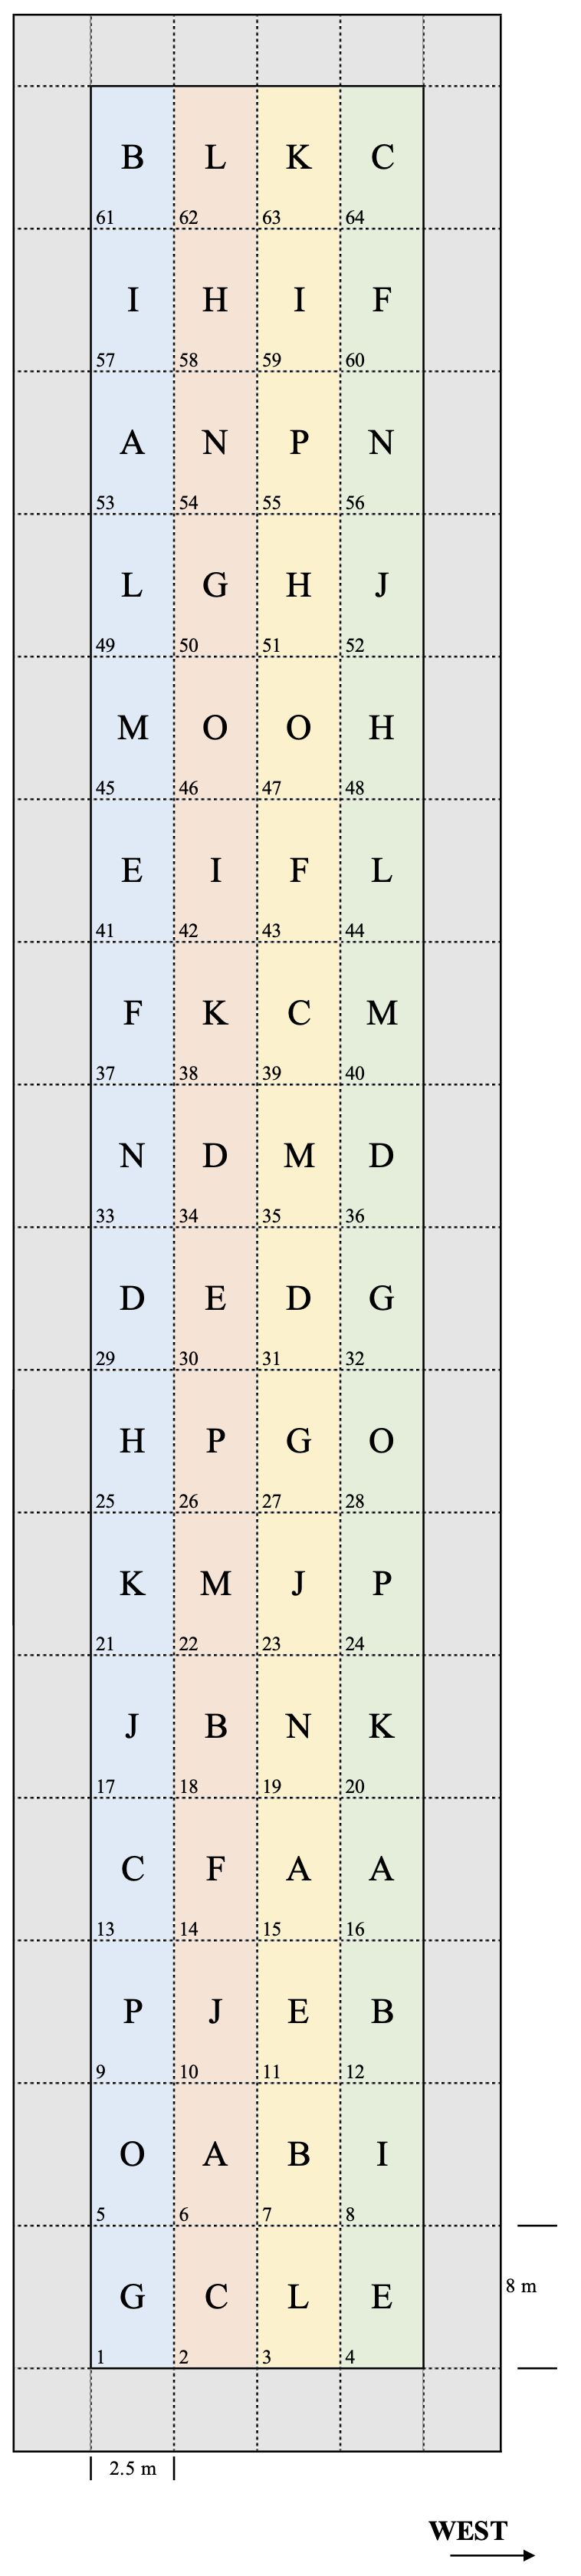
\includegraphics[width=0.3\linewidth,height=\textheight,keepaspectratio]{_images/Esercizio2.7.xls.png}

}

\caption{Randomised Complete Blocks Design (see Exercise 2.7)}

\end{figure}%

`agricolae'

\bookmarksetup{startatroot}

\chapter{Describing the Observations}\label{describing-the-observations}

\section{Describing nominal data}\label{describing-nominal-data}

Nominal data are produced by assigning the subjects to one of a set of
categories, such as dead/alive, germinated/ungerminated, red/blue/green,
and so on. For this data, especially when the number of categories is
higher than two, the statistics described in book Chapter 3 cannot be
used and different approaches need to be sought for their description.

The most widespread technique is to derive \textbf{absolute
frequencies}, that are the counts of individuals in each category; by
doing so, a \textbf{distribution of frequencies} is built.

As an example of nominal data we can take the `mtcars' dataset, that was
extracted from the 1974 Motor Trend US magazine and comprises 32 old
automobiles. The dataset is available in R and we show part of it in
table 3.2.

\begin{longtable}[]{@{}lrr@{}}
\caption{Part of the dataset `mtcars' in R, representing the
characteristics of 32 old automobiles; `vs' is the type of engine (0 for
V-shaped and 1 for straight engine) and `gear' is the number of forward
gears. More detail is given in the text.}\tabularnewline
\toprule\noalign{}
& vs & gear \\
\midrule\noalign{}
\endfirsthead
\toprule\noalign{}
& vs & gear \\
\midrule\noalign{}
\endhead
\bottomrule\noalign{}
\endlastfoot
Mazda RX4 & 0 & 4 \\
Mazda RX4 Wag & 0 & 4 \\
Datsun 710 & 1 & 4 \\
Hornet 4 Drive & 1 & 3 \\
Hornet Sportabout & 0 & 3 \\
Valiant & 1 & 3 \\
Duster 360 & 0 & 3 \\
Merc 240D & 1 & 4 \\
Merc 230 & 1 & 4 \\
Merc 280 & 1 & 4 \\
Merc 280C & 1 & 4 \\
Merc 450SE & 0 & 3 \\
Merc 450SL & 0 & 3 \\
Merc 450SLC & 0 & 3 \\
Cadillac Fleetwood & 0 & 3 \\
Lincoln Continental & 0 & 3 \\
Chrysler Imperial & 0 & 3 \\
Fiat 128 & 1 & 4 \\
Honda Civic & 1 & 4 \\
Toyota Corolla & 1 & 4 \\
Toyota Corona & 1 & 3 \\
Dodge Challenger & 0 & 3 \\
AMC Javelin & 0 & 3 \\
Camaro Z28 & 0 & 3 \\
Pontiac Firebird & 0 & 3 \\
Fiat X1-9 & 1 & 4 \\
Porsche 914-2 & 0 & 5 \\
Lotus Europa & 1 & 5 \\
Ford Pantera L & 0 & 5 \\
Ferrari Dino & 0 & 5 \\
Maserati Bora & 0 & 5 \\
Volvo 142E & 1 & 4 \\
\end{longtable}

The variable `vs' in `mtcars' takes the values 0 for V-shaped engine and
1 for straight engine. Obviously, the two values 0 and 1 are just used
to name the two categories and the resulting variable is purely nominal.
The absolute frequencies of cars in the two categories are, respectively
18 and 14 and they are easily obtained by a counting process. In R,
these absolute frequencies can be obtained by the \texttt{table()}
function, as we show in the box below.

\begin{Shaded}
\begin{Highlighting}[]
\FunctionTok{data}\NormalTok{(mtcars)}
\FunctionTok{table}\NormalTok{(mtcars}\SpecialCharTok{$}\NormalTok{vs)}
\end{Highlighting}
\end{Shaded}

\begin{verbatim}

 0  1 
18 14 
\end{verbatim}

The \textbf{relative frequencies} are obtained by dividing the absolute
frequencies by the total number of observations. These frequencies are,
respectively, 0.5625 and 0.4375 and, in R, they can be obtained by the
joint usage of the \texttt{table()} and \texttt{length()} functions,
where this latter returns the number of values in a vector.

\begin{Shaded}
\begin{Highlighting}[]
\FunctionTok{table}\NormalTok{(mtcars}\SpecialCharTok{$}\NormalTok{vs)}\SpecialCharTok{/}\FunctionTok{length}\NormalTok{(mtcars}\SpecialCharTok{$}\NormalTok{vs)}
\end{Highlighting}
\end{Shaded}

\begin{verbatim}

     0      1 
0.5625 0.4375 
\end{verbatim}

If we consider a variable where the classes can be logically ordered, we
can also calculate the \textbf{cumulative frequencies}, by summing up
the frequency for one class with the frequencies for all previous
classes. As an example we take the `gear' variable in the `mtcars'
dataset, showing the number of forward gears for each car. We can easily
see that 15 cars have 3 gears and 27 cars have 4 gears or less. In R,
cumulative sums can be calculated by using the \texttt{cumsum()}
function, as shown in the box below.

\begin{Shaded}
\begin{Highlighting}[]
\FunctionTok{cumsum}\NormalTok{(}\FunctionTok{table}\NormalTok{(mtcars}\SpecialCharTok{$}\NormalTok{gear))}
\end{Highlighting}
\end{Shaded}

\begin{verbatim}
 3  4  5 
15 27 32 
\end{verbatim}

\section{Binning/Bucketing}\label{binningbucketing}

In some circumstances, it may be convenient to `bin' a continuous
variable into a set of intervals. For example, if we have recorded the
ages of a big group of people, we can divide the scale into intervals of
five years (e.g., from 10 to 15, from 15 to 20 and so on) and,
eventually, assign each individual to the appropriate age class. Such a
technique is called \textbf{binning} or \textbf{bucketing}.

As an example, we can consider the `co2' dataset, that is included in
the base R installation. It contains 468 values of CO\_2\_ atmospheric
concentrations, expressed in parts per million, as observed at monthly
intervals in the US. With such a big dataset, the mean and standard
deviation are not sufficient to get a good feel for the data and it
would be important to have an idea of the shape of the dataset.
Therefore we can split the continuous scale into a series of intervals,
from 310 ppm to 370 ppm, with breaks every 10 ppm and count the
observations in each interval. In the box below, the function
\texttt{cut()} assigns each value to the corresponding interval (please
note the `breaks' argument, which sets the margins of each interval.
Intervals are, by default, left open and right-closed), while the
function \texttt{table()} calculates the frequencies.

\begin{Shaded}
\begin{Highlighting}[]
\FunctionTok{data}\NormalTok{(co2)}
\NormalTok{co2 }\OtherTok{\textless{}{-}} \FunctionTok{as.vector}\NormalTok{(co2)}
\FunctionTok{mean}\NormalTok{(co2)}
\end{Highlighting}
\end{Shaded}

\begin{verbatim}
[1] 337.0535
\end{verbatim}

\begin{Shaded}
\begin{Highlighting}[]
\FunctionTok{min}\NormalTok{(co2)}
\end{Highlighting}
\end{Shaded}

\begin{verbatim}
[1] 313.18
\end{verbatim}

\begin{Shaded}
\begin{Highlighting}[]
\FunctionTok{max}\NormalTok{(co2)}
\end{Highlighting}
\end{Shaded}

\begin{verbatim}
[1] 366.84
\end{verbatim}

\begin{Shaded}
\begin{Highlighting}[]
\CommentTok{\# binning}
\NormalTok{classes }\OtherTok{\textless{}{-}} \FunctionTok{cut}\NormalTok{(co2, }\AttributeTok{breaks =} \FunctionTok{c}\NormalTok{(}\DecValTok{310}\NormalTok{,}\DecValTok{320}\NormalTok{,}\DecValTok{330}\NormalTok{,}\DecValTok{340}\NormalTok{,}\DecValTok{350}\NormalTok{,}\DecValTok{360}\NormalTok{,}\DecValTok{370}\NormalTok{))}
\NormalTok{freq }\OtherTok{\textless{}{-}} \FunctionTok{table}\NormalTok{(classes)}
\NormalTok{freq}
\end{Highlighting}
\end{Shaded}

\begin{verbatim}
classes
(310,320] (320,330] (330,340] (340,350] (350,360] (360,370] 
       70       117        86        76        86        33 
\end{verbatim}

\section{Descriptive stats for distributions of
frequencies}\label{descriptive-stats-for-distributions-of-frequencies}

For nominal data, we can retrieve the \textbf{mode}, which is the class
with the highest frequency. For ordinal data, wherever distances between
classes are meaningful, and for discrete data, we can also calculate the
median and other percentiles, as well as the mean and other statistics
of spread (e.g., variance, standard deviation). The mean is calculated
as:

\[\mu = \frac{\sum\limits_{i = 1}^n f_i x_i}{\sum\limits_{i = 1}^n f_i}\]

where \(x_i\) is the value for the i-th class, and \(f_i\) is the
frequency for the same class. Likewise, the deviance, is calculated as:

\[SS = \sum\limits_{i = 1}^n f_i (x_i - \mu)^2\]

For example, considering the `gear' variable in Table 3.2, the average
number of forward gears is:

\[\frac{ 15 \times 3 + 12 \times 4 + 5 \times 5}{15 + 12 + 5} = 3.6875\]

while the deviance is:

\[SS = 15 \times (3 - 3.6875)^2 + 12 \times (4 - 3.6875)^2 + 5 \times (5 - 3.l875)^2 = 16.875\]

With interval data (binned data), descriptive statistics should be
calculated by using the raw data, if they are available. If they are
not, we can use the frequency distribution obtained from binning, by
assigning to each individual the central value of the interval class to
which it belongs. As an example, we can consider the distribution of
frequencies in Table 3.3, relating to the time (in minutes) taken to
complete a statistic assignment for a group of students in
biotechnology. We can see that the mean is equal to:

\[\frac{7.5 \times 1 + 12.5 \times 4 + 17.5 \times 3 + 22.5 \times 2}{10} = 15.5\]

\begin{longtable}[]{@{}ccc@{}}
\caption{Distribution of frequency for the time (in minutes) taken to
complete a statistic assignment for a group of students in
biotechnology}\tabularnewline
\toprule\noalign{}
Time interval & Central value & Count \\
\midrule\noalign{}
\endfirsthead
\toprule\noalign{}
Time interval & Central value & Count \\
\midrule\noalign{}
\endhead
\bottomrule\noalign{}
\endlastfoot
5 - 10 & 7.5 & 1 \\
10 - 15 & 12.5 & 4 \\
15 - 20 & 17.5 & 3 \\
20 - 25 & 22.5 & 2 \\
\end{longtable}

The calculation of the deviance is left as an exercise.

\section{Graphical representations of nominal
data}\label{graphical-representations-of-nominal-data}

A distribution of frequency can be represented by using a barplot, as
described in the main book. It can also be represented by using a `pie'
chart, drawn with \texttt{ggplot}. The coding consists of producing a
bar chart with stacked segments and rotating the coordinate system, as
shown in the box below.

\begin{Shaded}
\begin{Highlighting}[]
\FunctionTok{library}\NormalTok{(ggplot2)}
\NormalTok{dfr }\OtherTok{\textless{}{-}} \FunctionTok{data.frame}\NormalTok{(}\StringTok{"Class"} \OtherTok{=} \FunctionTok{names}\NormalTok{(freq),}
                  \StringTok{"Freq"} \OtherTok{=} \FunctionTok{as.numeric}\NormalTok{(freq))}
\FunctionTok{ggplot}\NormalTok{(}\AttributeTok{data =}\NormalTok{ dfr) }\SpecialCharTok{+}
  \FunctionTok{geom\_bar}\NormalTok{(}\FunctionTok{aes}\NormalTok{(}\AttributeTok{x =} \ConstantTok{NA}\NormalTok{, }\AttributeTok{y =}\NormalTok{ Freq, }\AttributeTok{fill =}\NormalTok{ Class),}
           \AttributeTok{stat=}\StringTok{"identity"}\NormalTok{, }\AttributeTok{position =} \StringTok{"fill"}\NormalTok{) }\SpecialCharTok{+}
  \FunctionTok{coord\_polar}\NormalTok{(}\StringTok{"y"}\NormalTok{, }\AttributeTok{start=}\DecValTok{0}\NormalTok{) }\SpecialCharTok{+}
  \FunctionTok{theme\_void}\NormalTok{() }\CommentTok{\# remove background, grid, numeric labels}
\end{Highlighting}
\end{Shaded}

\pandocbounded{\includegraphics[keepaspectratio]{03-DescriptiveStats_files/figure-pdf/unnamed-chunk-7-1.pdf}}

\section{Contingency tables}\label{contingency-tables}

When we have more than one cataegorical variable, we can summarise the
distribution of frequency by using two-way tables, usually known as
\textbf{contingency tables} or crosstabs. These tables can be created by
providing two or more vectors as arguments to the \texttt{table()}
function; it is important to keep in mind that, even if the resulting
table may resamble a matrix or a data.frame, a contingency table
represents a peculiar class in R, with several specific methods, that we
will explore later. The box below shows a contingency table that shows
the cross tabulation for `gear' and `vs' in `mtcars'.

\begin{Shaded}
\begin{Highlighting}[]
\FunctionTok{table}\NormalTok{(mtcars}\SpecialCharTok{$}\NormalTok{vs, mtcars}\SpecialCharTok{$}\NormalTok{gear)}
\end{Highlighting}
\end{Shaded}

\begin{verbatim}
   
     3  4  5
  0 12  2  4
  1  3 10  1
\end{verbatim}

Another interesting table is contained in the `datasets' package and is
named `HairEyeColor'. It shows the distribution of hair and eye color in
592 statistics students, depending on sex; both characters are expressed
in four classes, i.e.~black, brown, red and blond hair and brown, blue,
hazel and green eyes. Considering females, the contingency table is
reported in the following table and it is augmented with row and column
sums (see later).

\begin{longtable}[]{@{}lcccc@{}}
\caption{Distribution of hair and eye color for 313 female statistics
students, augmented with row and column sums. Dataset taken from R
package `datasets'}\tabularnewline
\toprule\noalign{}
& Brown eye & Blue eye & Hazel eye & Green eye \\
\midrule\noalign{}
\endfirsthead
\toprule\noalign{}
& Brown eye & Blue eye & Hazel eye & Green eye \\
\midrule\noalign{}
\endhead
\bottomrule\noalign{}
\endlastfoot
Black hair & 36 & 9 & 5 & 2 \\
Brown hair & 66 & 34 & 29 & 14 \\
Red hair & 16 & 7 & 7 & 7 \\
Blond hair & 4 & 64 & 5 & 8 \\
\end{longtable}

\subsection{Independence}\label{independence}

With a contingency table, we may be interested in assessing whether the
two variables show some sort of dependency relationship. In the previous
example, is there any relationship between the color of the eyes and the
color of the hair? If not, we say that the two variables are
independent. Independency is assessed by using the \(\chi^2\) statistic.

In order to make hand calculations easier, let's restrict our attention
to people with Black/Blond hair and Brown/Blue eyes. This `restricted'
contingency table is reported below and clearly shows that the vast
majority of people with black hair have brown eyes, while the vast
majority of people with blond hair have blue eyes. It would apper that
there is a strong association between the color of hair and the color of
eyes.

\begin{longtable}[]{@{}lccc@{}}
\caption{Excerpt from the previous table, considering (for the sake of
simplicity) only two color classes for both hair and
eyes}\tabularnewline
\toprule\noalign{}
& Brown eye & Blue eye & ROW SUMS \\
\midrule\noalign{}
\endfirsthead
\toprule\noalign{}
& Brown eye & Blue eye & ROW SUMS \\
\midrule\noalign{}
\endhead
\bottomrule\noalign{}
\endlastfoot
Black hair & 36 & 9 & 45 \\
Blond hair & 4 & 64 & 68 \\
COLUMN SUMS & 40 & 73 & 113 \\
\end{longtable}

In order to elucidate such an association, we can, as the first step
calculate the \emph{marginal frequencies}, i.e.~the sums of frequencies
by row and by column (please note that the entries of a contingency
table are called \emph{joint frequencies}). These sums are reported in
the Table above.

In total, we have 45 individuals with black hair, that is 45/113 × 100 =
39.8\% of the whole sample, while we have 68/113×100 = 60.2\% of
individuals with blond hair. If the two characters were really
independent, the above percentages should not change, depending on the
color of eyes; consequently, in the brown eyes group, the number of
individuals with black hair should be 15.93 (i.e., 39.8\% of 40), while
the number of individuals with blonde hair should be 24.08 (i.e.~60.2\%
of 40). From there, we could derive a full table of expected
frequencies, assuming complete independence between the two characters
(see below).

\begin{longtable}[]{@{}lcc@{}}
\caption{Expected counts of hair and eye color, assuming total lack of
dependency between the two characters.}\tabularnewline
\toprule\noalign{}
& Brown & Blue \\
\midrule\noalign{}
\endfirsthead
\toprule\noalign{}
& Brown & Blue \\
\midrule\noalign{}
\endhead
\bottomrule\noalign{}
\endlastfoot
Black & 15.93 & 29.07 \\
Blonde & 24.07 & 43.93 \\
\end{longtable}

The observed and expected values are different, which might indicate a
some sort of relationship between the two variables; for example, having
red hair might imply that we are more likely to have eyes of a certain
color. In order to quantify the discrepancy between the two tables, we
calculate the \(\chi^2\) stat, that is:

\[\chi ^2  = \sum \left[ \frac{\left( {f_o  - f_e } \right)^2 }{f_e } \right]\]

where \(f_o\) are the observed frequencies and \(f_e\) are the expected
frequencies. For this example:

\[\chi ^2  = \left[ \frac{\left( {36  - 15.93 } \right)^2 }{15.93} \right] + \left[ \frac{\left( {9  - 29.07 } \right)^2 }{129.07} \right] +\left[ \frac{\left( {4  - 24.07 } \right)^2 }{24.07 } \right] + \left[ \frac{\left( {64  - 43.93 } \right)^2 }{43.93 } \right] = 65.05\]

The final \(\chi^2\) value should be equal to 0 in case of independence
and it should increase as the relationship between the two variables
increases. With R, the chi square value is provided as an output of the
\texttt{summary()} method, applied to the table object.

\begin{Shaded}
\begin{Highlighting}[]
\NormalTok{tab }\OtherTok{\textless{}{-}} \FunctionTok{as.table}\NormalTok{(}\FunctionTok{matrix}\NormalTok{(}\FunctionTok{c}\NormalTok{(}\DecValTok{36}\NormalTok{, }\DecValTok{9}\NormalTok{, }\DecValTok{4}\NormalTok{, }\DecValTok{64}\NormalTok{), }\DecValTok{2}\NormalTok{, }\DecValTok{2}\NormalTok{, }\AttributeTok{byrow =} \ConstantTok{TRUE}\NormalTok{))}
\FunctionTok{summary}\NormalTok{(tab)}
\end{Highlighting}
\end{Shaded}

\begin{verbatim}
Number of cases in table: 113 
Number of factors: 2 
Test for independence of all factors:
    Chisq = 65.05, df = 1, p-value = 7.295e-16
\end{verbatim}

The \(\chi^2\) value needs to be compared with its maximum allawable
value, which is:

\[\max \left( \chi ^2 \right)  = n \cdot \min (r - 1,\,c - 1)\]

i.e.~the product between the number of subjects (\(n\)) and the minimum
value between the number of rows minus one and the number of columns
minus one (in our case, it is \(113 \times 1 = 113\)). This suggests
that the two variables are not independent. The square root of the ratio
between the observed chi square value and the maximum value is know as
the Cramer's V coefficient and it is more understandable than the chi
square, as it is always included between 0 and 1.

\begin{Shaded}
\begin{Highlighting}[]
\NormalTok{Vcram }\OtherTok{\textless{}{-}} \FunctionTok{sqrt}\NormalTok{(}\FunctionTok{summary}\NormalTok{(tab)}\SpecialCharTok{$}\NormalTok{statistic}\SpecialCharTok{/}\NormalTok{(}\FunctionTok{sum}\NormalTok{(tab) }\SpecialCharTok{*} \FunctionTok{min}\NormalTok{(}\FunctionTok{nrow}\NormalTok{(tab) }\SpecialCharTok{{-}} \DecValTok{1}\NormalTok{, }\FunctionTok{ncol}\NormalTok{(tab) }\SpecialCharTok{{-}} \DecValTok{1}\NormalTok{)))}
\NormalTok{Vcram}
\end{Highlighting}
\end{Shaded}

\begin{verbatim}
[1] 0.7587364
\end{verbatim}

\section{Questions and exercises}\label{questions-and-exercises}

\begin{enumerate}
\def\labelenumi{\arabic{enumi}.}
\tightlist
\item
  List and discuss the main statistics for nominal and ordinal variables
\item
  Describe and discuss briefly the chi square coefficient
\item
  A scientist ha compared the proportion of females in two random
  samples of insects treated with two different substances (A and B).
  With substance A, they found 275 males and 175 females, while, with
  substance B they found 326 males and 297 females. Considering these
  results, determine the degree of association between the two variables
  (sex and substance), in relation to the maximum and minimum allowable
  level for the selected statistic.
\item
  Load the csv file `students.csv' from
  \url{https://www.casaonofri.it/_datasets/students.csv}. This dataset
  relates to a number of students, their votes in several undergraduate
  exams and information on high school. Determine: (i) the absolute and
  relative frequencies for the different subjects; (ii) the frequency
  distribution of votes in three classes (bins): \textless24, 24-27,
  \textgreater27; (iii) whether the votes depend on the exam subject and
  (iv) whether the votes depend on the high school type.
\end{enumerate}

\bookmarksetup{startatroot}

\chapter{Cause-effect Relationships}\label{cause-effect-relationships}

\section{Assessing the `goodness of fit' for regression
models}\label{assessing-the-goodness-of-fit-for-regression-models}

\begin{enumerate}
\def\labelenumi{\arabic{enumi}.}
\tightlist
\item
  Coefficient of determination
\item
  AIC/BIC values
\end{enumerate}

To be developed, yet

\bookmarksetup{startatroot}

\chapter{Stochastic models}\label{stochastic-models}

\section{\texorpdfstring{List of
\emph{errata}}{List of errata}}\label{list-of-errata}

\begin{enumerate}
\def\labelenumi{\arabic{enumi}.}
\tightlist
\item
  In Example 5.2 the correct cause-effect relationship is
  \(C = C_0 \, 10^{−0.05\, t}\). Furthermore, in the first sentence of
  Page 93, the standard deviation is calculated as:
  \(4.22 \times 10\%\), so that the correct sentence should read:
  \emph{Assuming that the cause-effect relationship is reliable, the
  expected concentration at 20 days after the treatment should be 4.22
  ng g\textsuperscript{−1}. (Code Box 5.5). However, the observed result
  depends on the experimental error, which is a random, unpredictable
  event; if we assume that the probability function for the observed
  concentration is Gaussian, with a mean of 4.22 and a standard
  deviation of 0.422 (i.e., 4.22 \(\times\) 10\%), the probability of
  obtaining a measure of 3 ng g\textsuperscript{−1}. or lower is less
  than 0.2\%, which is a relatively unlikely event.}
\end{enumerate}

\bookmarksetup{startatroot}

\chapter{Statistical Inference}\label{statistical-inference}

\section{\texorpdfstring{List of
\emph{errata}}{List of errata}}\label{list-of-errata-1}

\begin{enumerate}
\def\labelenumi{\arabic{enumi}.}
\tightlist
\item
  At page 101, in Code box 6.1, we are reconsidering Example 5.3, not
  5.2
\end{enumerate}

\bookmarksetup{startatroot}

\chapter{Making Decisions under
uncertainty}\label{making-decisions-under-uncertainty}

Nothing to add, yet

\bookmarksetup{startatroot}

\chapter{Checking fitted models}\label{checking-fitted-models}

\section{\texorpdfstring{List of
\emph{errata}}{List of errata}}\label{list-of-errata-2}

\begin{enumerate}
\def\labelenumi{\arabic{enumi}.}
\tightlist
\item
  At page 136, an example of the Levene's test is given in Code Box 8.1,
  not 8.3
\end{enumerate}

\bookmarksetup{startatroot}

\chapter{Linear/nonlinear combinations of model
parameters}\label{linearnonlinear-combinations-of-model-parameters}

\section{Multiplicity corrections in
`emmeans'}\label{multiplicity-corrections-in-emmeans}

In the main book, at page 166 and earlier I have made the point that,
with pairwise comparisons and, more generally, whenever simoultanous
statistical tests are performed, it is necessary to provide P-values
that account for the familywise error rate, i.e., the probability of
committing at least one wrong rejection within the whole family of
simuoltaneous tests (i.e., adjusted P-values).

With linear/nonlinear combinations of model parameters, a single test is
usually based on the ratio between the combination (e.g., the difference
between two means) and its standard error (t-test), which is supposed to
follow a univariate t-distribution, when the null hypothesis is true.
Consequently, when we have several simoultaneous t-tests, the vector of
all the t-ratios can be supposed to follow a multivariate
t-distribution, under the hypothesis that the null is true for all
simoultaneous tests (Bretz et al., 2011). Therefore, adjusted P-values
can be obtained by using the probability function of a multivariate
t-distribution, although the calculations can be rather difficult.

As an example, let's reconsider the `mixture' data, which we have used
in Chapter 9 of the main book: three herbicide mixtures and the
untreated control were tested for their weed control ability against an
important weed in tomato, i.e.~\emph{Solanum nigrum}. In the code below,
we load the data, fit a one-way ANOVA model, using the weight of weed
plants per pot as the response variable and the herbicide treatment as
the explanatory factor. For the sake of simplicity, we omit the usual
check for basic assumptions (see the main book); the ANOVA table shows
that the treatment effect is significant and, thus, we proceed to
comparing the means of treatments in a pairwise fashion. The P-values
shown below do not account for the familiwise error rate, but only for
the comparisonwise error rate; those P-values can be reproduced by using
the probability function of a univariate Student's t-distribution.

\begin{Shaded}
\begin{Highlighting}[]
\FunctionTok{library}\NormalTok{(statforbiology)}
\end{Highlighting}
\end{Shaded}

\begin{verbatim}
Loading required package: drc
\end{verbatim}

\begin{verbatim}
Loading required package: MASS
\end{verbatim}

\begin{verbatim}

'drc' has been loaded.
\end{verbatim}

\begin{verbatim}
Please cite R and 'drc' if used for a publication,
\end{verbatim}

\begin{verbatim}
for references type 'citation()' and 'citation('drc')'.
\end{verbatim}

\begin{verbatim}

Attaching package: 'drc'
\end{verbatim}

\begin{verbatim}
The following objects are masked from 'package:stats':

    gaussian, getInitial
\end{verbatim}

\begin{Shaded}
\begin{Highlighting}[]
\FunctionTok{library}\NormalTok{(emmeans)}
\end{Highlighting}
\end{Shaded}

\begin{verbatim}
Welcome to emmeans.
Caution: You lose important information if you filter this package's results.
See '? untidy'
\end{verbatim}

\begin{Shaded}
\begin{Highlighting}[]
\FunctionTok{library}\NormalTok{(multcomp)}
\end{Highlighting}
\end{Shaded}

\begin{verbatim}
Loading required package: mvtnorm
\end{verbatim}

\begin{verbatim}
Loading required package: survival
\end{verbatim}

\begin{verbatim}
Loading required package: TH.data
\end{verbatim}

\begin{verbatim}

Attaching package: 'TH.data'
\end{verbatim}

\begin{verbatim}
The following object is masked from 'package:MASS':

    geyser
\end{verbatim}

\begin{Shaded}
\begin{Highlighting}[]
\NormalTok{dataset }\OtherTok{\textless{}{-}} \FunctionTok{getAgroData}\NormalTok{(}\StringTok{"mixture"}\NormalTok{)}
\NormalTok{dataset}\SpecialCharTok{$}\NormalTok{Treat }\OtherTok{\textless{}{-}} \FunctionTok{factor}\NormalTok{(dataset}\SpecialCharTok{$}\NormalTok{Treat)}
\NormalTok{model }\OtherTok{\textless{}{-}} \FunctionTok{lm}\NormalTok{(Weight }\SpecialCharTok{\textasciitilde{}}\NormalTok{ Treat, }\AttributeTok{data =}\NormalTok{ dataset)}
\FunctionTok{anova}\NormalTok{(model)}
\end{Highlighting}
\end{Shaded}

\begin{verbatim}
Analysis of Variance Table

Response: Weight
          Df  Sum Sq Mean Sq F value    Pr(>F)    
Treat      3 1089.53  363.18  23.663 2.509e-05 ***
Residuals 12  184.18   15.35                      
---
Signif. codes:  0 '***' 0.001 '**' 0.01 '*' 0.05 '.' 0.1 ' ' 1
\end{verbatim}

\begin{Shaded}
\begin{Highlighting}[]
\NormalTok{groupMeans }\OtherTok{\textless{}{-}} \FunctionTok{emmeans}\NormalTok{(model, }\SpecialCharTok{\textasciitilde{}}\NormalTok{Treat)}
\NormalTok{tab }\OtherTok{\textless{}{-}} \FunctionTok{contrast}\NormalTok{(groupMeans, }\AttributeTok{method =} \StringTok{"pairwise"}\NormalTok{, }\AttributeTok{adjust =} \StringTok{"none"}\NormalTok{)}
\NormalTok{tab}
\end{Highlighting}
\end{Shaded}

\begin{verbatim}
 contrast                         estimate   SE df t.ratio p.value
 Metribuzin__348 - Mixture_378        4.05 2.77 12   1.461  0.1697
 Metribuzin__348 - Rimsulfuron_30    -7.68 2.77 12  -2.774  0.0168
 Metribuzin__348 - Unweeded         -17.60 2.77 12  -6.352 <0.0001
 Mixture_378 - Rimsulfuron_30       -11.73 2.77 12  -4.235  0.0012
 Mixture_378 - Unweeded             -21.64 2.77 12  -7.813 <0.0001
 Rimsulfuron_30 - Unweeded           -9.91 2.77 12  -3.578  0.0038
\end{verbatim}

\begin{Shaded}
\begin{Highlighting}[]
\CommentTok{\# The P{-}value is obtained from the univariate t distribution (two{-}tails test)}
\NormalTok{abst }\OtherTok{\textless{}{-}} \FunctionTok{abs}\NormalTok{(}\FunctionTok{as.data.frame}\NormalTok{(tab)}\SpecialCharTok{$}\NormalTok{t.ratio)}
\DecValTok{2} \SpecialCharTok{*} \FunctionTok{pt}\NormalTok{(abst, }\DecValTok{12}\NormalTok{, }\AttributeTok{lower.tail =} \ConstantTok{FALSE}\NormalTok{)}
\end{Highlighting}
\end{Shaded}

\begin{verbatim}
[1] 1.696785e-01 1.683167e-02 3.651239e-05 1.157189e-03 4.782986e-06
[6] 3.794451e-03
\end{verbatim}

In order to obtain familywise error rates, we should switch from the
univariate to the multivariate t-distribution. For example, let's
consider the first t-ratio in the previous Code Box (t = 1.461); we
should ask ourselves: ``what is the probability of obtaining a t-ratio
as extreme or more extreme than 1.461 from a multivariate t-distribution
with 6 dimensions (i.e., the number of simoultaneous tests)?''. In this
calculation we should also consider that the 6 tests are correlated, at
least to some extent, due to fact the they, e.g., use the same error
term at the denominator. In the simplest case (homoscedasticity and
balanced data), the correlation is equal to 0.5 for all pairwise
comparisons.

In formers time, when the computing power used to be limiting,
calculating probabilities from the multivariate t-distribution was a
daunting task. However, for some specific cases (e.g., linear models
with homoscedastic and balanced data), adjusted P-values could be
calculated by exploiting the distribution of the Studentised Range (so
called `tukey' method), which is the default method in the
\texttt{contrast()} function of the \texttt{emmeans} package, as shown
in the following Code box.

\begin{Shaded}
\begin{Highlighting}[]
\NormalTok{tab }\OtherTok{\textless{}{-}} \FunctionTok{contrast}\NormalTok{(groupMeans, }\AttributeTok{method =} \StringTok{"pairwise"}\NormalTok{)}
\CommentTok{\# tab \textless{}{-} contrast(groupMeans, method = "pairwise", adjust = "tukey") \# same as above}
\NormalTok{tab}
\end{Highlighting}
\end{Shaded}

\begin{verbatim}
 contrast                         estimate   SE df t.ratio p.value
 Metribuzin__348 - Mixture_378        4.05 2.77 12   1.461  0.4885
 Metribuzin__348 - Rimsulfuron_30    -7.68 2.77 12  -2.774  0.0698
 Metribuzin__348 - Unweeded         -17.60 2.77 12  -6.352  0.0002
 Mixture_378 - Rimsulfuron_30       -11.73 2.77 12  -4.235  0.0055
 Mixture_378 - Unweeded             -21.64 2.77 12  -7.813 <0.0001
 Rimsulfuron_30 - Unweeded           -9.91 2.77 12  -3.578  0.0173

P value adjustment: tukey method for comparing a family of 4 estimates 
\end{verbatim}

\begin{Shaded}
\begin{Highlighting}[]
\CommentTok{\# The P{-}value is obtained from the Studentised Range Distribution (two{-}tails test)}
\NormalTok{abst }\OtherTok{\textless{}{-}} \FunctionTok{abs}\NormalTok{(}\FunctionTok{as.data.frame}\NormalTok{(tab)}\SpecialCharTok{$}\NormalTok{t.ratio)}
\FunctionTok{ptukey}\NormalTok{(}\FunctionTok{sqrt}\NormalTok{(}\DecValTok{2}\NormalTok{) }\SpecialCharTok{*}\NormalTok{ abst, }\DecValTok{4}\NormalTok{, }\DecValTok{12}\NormalTok{, }\AttributeTok{lower.tail =} \ConstantTok{FALSE}\NormalTok{)}
\end{Highlighting}
\end{Shaded}

\begin{verbatim}
[1] 4.884620e-01 6.981178e-02 1.853807e-04 5.501451e-03 2.473776e-05
[6] 1.725725e-02
\end{verbatim}

This simple method gives exact familywise error rates with balanced data
(which is the vast majority in designed field experiments in
agriculture) and works fairly well with some small degree of unbalance.
Considering the traditional Multiple Comparison Testing procedures, the
previous approach leads to the same results as the Tukey's HSD (for
balanced data) and to the Tukey-Kramer test (for unbalanced data).

In more recent times, it has become possible to directly calculate
probabilities from the multivariate t-distribution, which is handy, as
it provides a more general approach to obtaining familywise error rates.
Such a distribution is available in the `mvtnorm' package as the
\texttt{pmvt()} function: we need to define, for each dimension, the
interval for which we want to calculate the probability (in this case,
for the first t-ratio such an interval is: \(\pm 1.461081\)), the number
of degrees of freedom (12) and the correlation matrix for the linear
combinations, that can be directly retrieved from the `emmGrid' object.
The code below shows the calculations; the amount `plev' represents the
probability of sampling within the interval (none of the six nulls is
wrongly rejected), while the familywise error rate corresponds to the
probability of sampling outside the interval (at least one null is
wrongly rejected), that is obtained by subtraction.

\begin{Shaded}
\begin{Highlighting}[]
\FunctionTok{library}\NormalTok{(mvtnorm)}
\NormalTok{t1 }\OtherTok{\textless{}{-}} \FunctionTok{abs}\NormalTok{(}\FunctionTok{as.data.frame}\NormalTok{(tab)}\SpecialCharTok{$}\NormalTok{t.ratio)[}\DecValTok{1}\NormalTok{]}
\NormalTok{ncontr }\OtherTok{\textless{}{-}} \DecValTok{6}
\NormalTok{corMat }\OtherTok{\textless{}{-}} \FunctionTok{cov2cor}\NormalTok{(}\FunctionTok{vcov}\NormalTok{(tab))}
\NormalTok{plev }\OtherTok{\textless{}{-}} \FunctionTok{pmvt}\NormalTok{(}\AttributeTok{lower =} \FunctionTok{rep}\NormalTok{(}\SpecialCharTok{{-}}\NormalTok{t1, ncontr), }\AttributeTok{upper=}\FunctionTok{rep}\NormalTok{(t1, ncontr), }\AttributeTok{df =} \DecValTok{12}\NormalTok{,}
     \AttributeTok{corr =}\NormalTok{ corMat)[}\DecValTok{1}\NormalTok{]}
\DecValTok{1} \SpecialCharTok{{-}}\NormalTok{ plev}
\end{Highlighting}
\end{Shaded}

\begin{verbatim}
[1] 0.4884756
\end{verbatim}

The above function emplyes numerical calculation methods and, thus, the
results are not fully reproducible. However, it is easy to see that they
are asymptotically equivalent to theose obtained with the `tukey'
adjustment method. In R, such an approach can be obtained by using the
\texttt{adjust\ =\ "mvt"} argument.

\begin{Shaded}
\begin{Highlighting}[]
\NormalTok{tab }\OtherTok{\textless{}{-}} \FunctionTok{contrast}\NormalTok{(groupMeans, }\AttributeTok{method =} \StringTok{"pairwise"}\NormalTok{, }\AttributeTok{adjust =} \StringTok{"mvt"}\NormalTok{)}
\NormalTok{tab}
\end{Highlighting}
\end{Shaded}

\begin{verbatim}
 contrast                         estimate   SE df t.ratio p.value
 Metribuzin__348 - Mixture_378        4.05 2.77 12   1.461  0.4884
 Metribuzin__348 - Rimsulfuron_30    -7.68 2.77 12  -2.774  0.0696
 Metribuzin__348 - Unweeded         -17.60 2.77 12  -6.352  0.0002
 Mixture_378 - Rimsulfuron_30       -11.73 2.77 12  -4.235  0.0053
 Mixture_378 - Unweeded             -21.64 2.77 12  -7.813 <0.0001
 Rimsulfuron_30 - Unweeded           -9.91 2.77 12  -3.578  0.0172

P value adjustment: mvt method for 6 tests 
\end{verbatim}

Due to its complexity, this method is not recommended for pairwise
comparisons with balanced experiments, while it can turn out useful in
other cases, for example with strongly unbalanced data.

\bookmarksetup{startatroot}

\chapter{Putting everything together}\label{putting-everything-together}

No other case-studies, yet

\bookmarksetup{startatroot}

\chapter{Extending regression models}\label{extending-regression-models}

No other case-studies, yet

\bookmarksetup{startatroot}

\chapter{A brief intro to mixed
models}\label{a-brief-intro-to-mixed-models}

No additions, yet

\bookmarksetup{startatroot}

\chapter{Appendix: Updated list of
datasets}\label{appendix-updated-list-of-datasets}

Apart from those listed in the book, the package \texttt{statforbiology}
contains many other dataset and the list is continuously updated. In
this section you will find the full list of available datasets.

\section*{\texorpdfstring{\texttt{adjuvantsLS}}{adjuvantsLS}}\label{adjuvantsls}
\addcontentsline{toc}{section}{\texttt{adjuvantsLS}}

\markright{\texttt{adjuvantsLS}}

An experiment to compare three adjuvants (ammonium sulfate, mineral oil,
non-ionic surfactant, and a control with no adjuvant) for rimsulfuron,
which is a herbicide for weed control in maize. The experiment was
designed as a Latin square with five replicates (Onofri, unpublished
data), and the resulting dataset was slightly modified to make it more
suitable for teaching purposes.

\begin{enumerate}
\def\labelenumi{\arabic{enumi}.}
\tightlist
\item
  Herbicide (character): herbicide name
\item
  Adjuvant (character): adjuvant name
\item
  Dose (character): dose of the herbicide + adjuvant
\item
  Code (character): code for the adjuvants
\item
  Plot (numerical coding): code for the plots
\item
  Column (numerical coding): code for the column in the Latin square
  grid
\item
  Row (numerical coding): code for the row in the Latin square grid
\item
  Columns 8 to 23 (character): each column is a weed (identified by the
  respective Bayer code), and the values represent the abundances
  (Braun-Blanquet codes)
\item
  Yield (numeric): crop yield (100 kg per hectare)
\item
  Height (numeric): crop height (cm)
\end{enumerate}

\section*{\texorpdfstring{\texttt{alfalfa3years}}{alfalfa3years}}\label{alfalfa3years}
\addcontentsline{toc}{section}{\texttt{alfalfa3years}}

\markright{\texttt{alfalfa3years}}

A genotype experiment in alfalfa (Ligabue et al. 2009) to compare 20
genotypes in central Italy (medium Tiber Valley). The experiment was
laid out as an RCBD with four replicates and the total yearly forage
yield (sum of 3-4 cuts per year) was measured in each plot over 3 years
(from 2006 to 2008).

\begin{enumerate}
\def\labelenumi{\arabic{enumi}.}
\tightlist
\item
  Plot (numeric): code for the plot
\item
  Block (numeric): code for the block
\item
  Genotype (character): name of the genotype
\item
  Year (numeric): year when yield was measured
\item
  Yield (numeric): total yearly forage yield (sum of 3-4 cuts per year;
  in tons per hectare of dry matter)
\end{enumerate}

\section*{\texorpdfstring{\texttt{Ammi94}}{Ammi94}}\label{ammi94}
\addcontentsline{toc}{section}{\texttt{Ammi94}}

\markright{\texttt{Ammi94}}

A field experiment to evaluate the effect of different densities of
\emph{Ammi majus} on the achene yield of sunflower was performed in 1984
and published by Onofri and Tei (1994a). The values represent the means
of 4 replicates.

\begin{enumerate}
\def\labelenumi{\arabic{enumi}.}
\tightlist
\item
  Density (numeric): number of weed plants per square meter
\item
  Yield (numeric): sunflower yield in tons per hectare
\end{enumerate}

\section*{\texorpdfstring{\texttt{Ammi94\_YL}}{Ammi94\_YL}}\label{ammi94_YL}
\addcontentsline{toc}{section}{\texttt{Ammi94\_YL}}

\markright{\texttt{Ammi94\_YL}}

This dataset provides the results of a field experiment to evaluate the
effect of different densities of \emph{Ammi majus} on the achene yield
of sunflower. This experiment represents the repetition in time (2 years
later) of the experiment reported in the dataset `Ammi94' and contains
the full dataset (with replicates). These results were also published in
Onofri and Tei (1994a). The values represent the means of 4 replicates.

\begin{enumerate}
\def\labelenumi{\arabic{enumi}.}
\tightlist
\item
  Density (numeric): number of weed plants per square meter
\item
  Block (numeric): code for the blocks
\item
  Yield (numeric): sunflower yield in tons per hectare
\item
  Yield (numeric): sunflower yield in percentage of the average yield
  with no weeds
\item
  Yield loss (numeric): Yield loss with respect to the control with no
  weeds
\end{enumerate}

\section*{\texorpdfstring{\texttt{augmentedFactorial}}{augmentedFactorial}}\label{augmentedFactorial}
\addcontentsline{toc}{section}{\texttt{augmentedFactorial}}

\markright{\texttt{augmentedFactorial}}

An experiment to compare two herbicides (rimsulfuron and dicamba) at two
rates (HIGH and LOW) and with four adjuvant treatments (surfactant,
frigate, mineral oil and no adjuvant). Aside this fully crossed
structure, we introduced the untreated and hand-weeded controls. The
design is in complete blocks and it is termed `augmented factorial',
because some extra treatment levels has been included beyond the crossed
factorial structure.

\begin{enumerate}
\def\labelenumi{\arabic{enumi}.}
\tightlist
\item
  Plot (numerical coding): plot number
\item
  Herbicide (character): name of herbicides or controls
\item
  Adjuvant (character): adjuvant name
\item
  DoseF (character): code for the herbicide dose
\item
  Block (numerical coding): code for the block
\item
  Yield (numeric): maize yield (tons per hectare)
\end{enumerate}

\section*{\texorpdfstring{\texttt{BBsurvey}}{BBsurvey}}\label{BBsurvey}
\addcontentsline{toc}{section}{\texttt{BBsurvey}}

\markright{\texttt{BBsurvey}}

A field experiment aiming to compare the weed control abilities of nine
post-emergence herbicides against \emph{Sorghum halepense} in maize.
Three weeks after the treatment, the cover-abundance of \emph{S.
halepense} was visually recorded in six classes, using the
Braun-Blanquet method (Braun-Blanquet 1964).

\begin{enumerate}
\def\labelenumi{\arabic{enumi}.}
\tightlist
\item
  Plot (numeric): code for the plot
\item
  Herbicide (character): code for the herbicide
\item
  BBscore (character): Braun-Blanquet score (0, +, 1, 2, 3, 4, 5)
\item
  L (numeric): lower limit of the ground covering class (\%)
\item
  U (numeric): upper limit of the ground covering class (\%)
\item
  midPoint (numeric): centre of each ground covering class (\%)
\end{enumerate}

\section*{\texorpdfstring{\texttt{beet}}{beet}}\label{beet}
\addcontentsline{toc}{section}{\texttt{beet}}

\markright{\texttt{beet}}

A split-plot tillage experiment in sugarbeet, where three types of
tillage (minimum tillage = MIN; shallow plowing = SP; deep plowing = DP)
and two types of chemical weed control methods (broadcast = TOT;
in-furrow = PART) were compared in four complete blocks with three
main-plots per block, split into two sub-plots per main-plot; the three
types of tillage were randomly allocated to the main-plots in each
block, while the two weed control treatments were randomly allocated to
the sub-plots within each main-plot (Bianchi, 1992; unpublished data).

\begin{enumerate}
\def\labelenumi{\arabic{enumi}.}
\tightlist
\item
  Tillage (character): tillage method
\item
  WeedControl (character): weed control method
\item
  Block (numeric): code for the block
\item
  Yield (numeric): sugarbeet root yield in tons per hectare
\end{enumerate}

\section*{\texorpdfstring{\texttt{beetGrowth}}{beetGrowth}}\label{beetgrowth}
\addcontentsline{toc}{section}{\texttt{beetGrowth}}

\markright{\texttt{beetGrowth}}

An experiment in which sugarbeet was grown either weed-free, or
weed-infested (Covarelli and Onofri 1998). Crop weight per unit area (in
kg/ha) was measured at six different timings (in Days After Emergence;
DAE), using destructive methods from independent plots. The experiment
was conducted using a completely randomized design with three
replicates.

\begin{enumerate}
\def\labelenumi{\arabic{enumi}.}
\tightlist
\item
  DAE (numeric): Day After Emergence
\item
  Infested (numeric): Crop Dry Weight in weed-infested plots (kg/ha)
\item
  WeedFree (numeric): Crop Dry Weight in weed-free plots (kg/ha)
\end{enumerate}

\section*{\texorpdfstring{\texttt{brassica}}{brassica}}\label{brassica}
\addcontentsline{toc}{section}{\texttt{brassica}}

\markright{\texttt{brassica}}

A short-term pot-bioassay to determine the phytotoxicity of imazethapyr
was performed in hydroponic solution, using quartz-sand as a non
sorptive media. The assay was performed at the `Institut für
Unkrautforschung der Biologischen Bundesanstalt' (Braunschweig, Germany)
and the methods are described in Stalder and Pestemer (1980). The test
plant was \emph{Brassica rapa} and the results were published by Onofri
(1994).

\begin{enumerate}
\def\labelenumi{\arabic{enumi}.}
\tightlist
\item
  Dose (numeric): Herbicide concentration in soil solution (as mg/L)
\item
  FW (numeric): Fresh weight of the test plant as grams per pot.
\end{enumerate}

\section*{\texorpdfstring{\texttt{citrusGrove} or
\texttt{speciesArea}}{citrusGrove or speciesArea}}\label{citrusgrove-or-speciesarea}
\addcontentsline{toc}{section}{\texttt{citrusGrove} or
\texttt{speciesArea}}

\markright{\texttt{citrusGrove} or \texttt{speciesArea}}

An experiment was conducted in a citrus grove in Sicily (Southern Italy)
to determine the species-area relationship for the local weed community.
In this study, a nested-plot survey was employed (Muller-Dumbois and
Ellenberg 1974) where the number of weed species was counted in a plot
of 1 m\textsuperscript{2} surface and the sampling area was
progressively doubled in size. At each step, the number of new weed
species was counted. The dataset is taken from Cristaudo et al. (2015).

\begin{enumerate}
\def\labelenumi{\arabic{enumi}.}
\tightlist
\item
  Area (numeric): sampled area (in square meters)
\item
  numSpecies (numeric): count of the number of species
\end{enumerate}

\section*{\texorpdfstring{\texttt{crosses}}{crosses}}\label{crosses}
\addcontentsline{toc}{section}{\texttt{crosses}}

\markright{\texttt{crosses}}

An experiment to compare nine maize hybrids, obtained from three
pollinating inbred lines (A1, A2, and A3), each one crossed with three
different female inbred lines (A1 was crossed with B1, B2, and B3, A2
was crossed with B4, B5, and B6, while A3 was crossed B7, B8, and B9).
The experiment was laid out as complete blocks with four replicates (36
subjects in total). The dataset was generated through Monte Carlo
simulation.

\begin{enumerate}
\def\labelenumi{\arabic{enumi}.}
\tightlist
\item
  Male (character): pollinating line
\item
  Female (character): female line
\item
  Block (numeric): code for the blocks
\item
  Yield (numeric): maize yield (in tons per hectare)
\end{enumerate}

\section*{\texorpdfstring{\texttt{fabaBeanSplitMet}}{fabaBeanSplitMet}}\label{fabaBeanSplitMet}
\addcontentsline{toc}{section}{\texttt{fabaBeanSplitMet}}

\markright{\texttt{fabaBeanSplitMet}}

Six faba bean genotypes were tested at two sowing times using a
split-plot design in four complete blocks. Sowing times were randomized
to main-plots within blocks, and genotypes were randomized to sub-plots
within main-plots and blocks. The experiment was repeated in three years
and two locations of Central Italy. The dataset was taken from Stagnari
et al. (2007).

\begin{enumerate}
\def\labelenumi{\arabic{enumi}.}
\tightlist
\item
  Location (character): name of the location
\item
  Season (numeric): year of harvest
\item
  Sowing (character): sowing time
\item
  Genotype (character): name of the genotype
\item
  Block (numeric): code for the block in each experiment
\item
  Yield (numeric): crop grain yield in tons per hectare
\end{enumerate}

\section*{\texorpdfstring{\texttt{failureTimes}}{failureTimes}}\label{failuretimes}
\addcontentsline{toc}{section}{\texttt{failureTimes}}

\markright{\texttt{failureTimes}}

An experiment to record the failure time of heating systems as affected
by four different operating temperatures. The design was completely
randomized with six replicates, and the number of hours before failure
was measured. The dataset is taken from W. (1972).

\begin{enumerate}
\def\labelenumi{\arabic{enumi}.}
\tightlist
\item
  Temp (numeric): testing temperature (in \(^{\circ}\)F)
\item
  Hours\_to\_failure (numeric): number of hours before failure
\end{enumerate}

\section*{\texorpdfstring{\texttt{FertilizationTiming}}{FertilizationTiming}}\label{fertilizationtiming}
\addcontentsline{toc}{section}{\texttt{FertilizationTiming}}

\markright{\texttt{FertilizationTiming}}

A field experiment to evaluate the effect of fertilization timing
(early, optimal, late) on two genotypes (A and B). The experiment was
laid out as an RCBD, and the response represents the amount of absorbed
nitrogen by the plant (simulated data).

\begin{enumerate}
\def\labelenumi{\arabic{enumi}.}
\tightlist
\item
  Timing (character): timing of fertilization (early, optimal, late)
\item
  Genotype (character): genotype
\item
  Block (numeric): code for the block
\item
  Nabs (numeric): amount of absorbed nitrogen
\end{enumerate}

\section*{\texorpdfstring{\texttt{FGP\_rape}}{FGP\_rape}}\label{fgp_rape}
\addcontentsline{toc}{section}{\texttt{FGP\_rape}}

\markright{\texttt{FGP\_rape}}

An experiment where the germination of three genotypes of oilseed rape
was assessed in controlled conditions, at 20 \(^{\circ}\)C, according to
an RCBD with six replicates. One replicate per genotype, consisting of a
Petri dish with 50 seeds, was put in each of six shelves inside the
oven. The number of germinated seeds was counted 15 days after the start
of the assay and expressed as the Final Proportion of Germinated seeds
(FGP). The assay was repeated twice in different and independent ovens
with the same experimental design. The dataset is taken from Pace et al.
(2012).

\begin{enumerate}
\def\labelenumi{\arabic{enumi}.}
\tightlist
\item
  Dish (numeric): code for the Petri dish
\item
  Run (numeric coding): code for the run
\item
  Shelf (numeric): code for the shelf
\item
  Species (character): plant species
\item
  Genotype (character): genotype
\item
  FGP (numeric): Final Germinated Proportion in each dish
\end{enumerate}

\section*{\texorpdfstring{\texttt{floristicData1}}{floristicData1}}\label{floristicData1}
\addcontentsline{toc}{section}{\texttt{floristicData1}}

\markright{\texttt{floristicData1}}

An experiment where the weed flora composed by 8 weed species was
recorded in 120 plots, included in a three-factor factorial experiment
in a randomised blocks design. The counts of weeds are reported and the
dataset was modified from Scavo et al. (2020).

\begin{enumerate}
\def\labelenumi{\arabic{enumi}.}
\tightlist
\item
  F1 to F3 (character): the three experimental factors, respectively
  with 5, 2 and 3 levels
\item
  Rep (character): the blocks
\item
  SP1 to SP8 (numeric): the counts for the eight weed species
\end{enumerate}

\section*{\texorpdfstring{\texttt{heights}}{heights}}\label{heights}
\addcontentsline{toc}{section}{\texttt{heights}}

\markright{\texttt{heights}}

Highly unbalanced dataset, containing the height (cm) and yield (t/ha)
of 20 maize plants belonging to 4 different genotypes. The dataset was
generated through Monte Carlo simulation.

\begin{enumerate}
\def\labelenumi{\arabic{enumi}.}
\tightlist
\item
  Id (numeric): code for the plot
\item
  var (character): code for the genotype
\item
  height (numeric): crop height (cm)
\item
  yield (numeric): crop yield (t/ha)
\end{enumerate}

\section*{\texorpdfstring{\texttt{Hordeum\_GR}}{Hordeum\_GR}}\label{Hordeum_GR}
\addcontentsline{toc}{section}{\texttt{Hordeum\_GR}}

\markright{\texttt{Hordeum\_GR}}

The germination rates of \emph{Hordeum spontaneum} were studied, as
affected by the environmental temperatures. This data was derived by
germination assays at different temperatures, by using the dataset in
Mesgaran et al. (2017), with some slight modifications of the technique
described in that manuscript.

\begin{enumerate}
\def\labelenumi{\arabic{enumi}.}
\tightlist
\item
  Temp (numeric): Environmental temperature (in °C)
\item
  T50 (numeric): Median time to germination for the seed lot under study
  (in hours)
\item
  GR50 (numeric): Median germination rate (as hours\textsuperscript{-1})
\end{enumerate}

\section*{\texorpdfstring{\texttt{insects}}{insects}}\label{insects}
\addcontentsline{toc}{section}{\texttt{insects}}

\markright{\texttt{insects}}

An experiment in which tobacco plants were treated with three different
insecticides was conducted using a completely randomized design with
five replicates (resulting in a total of fifteen plants). The number of
insects over the surface of leaves in each plant was counted three weeks
after the treatments.

\begin{enumerate}
\def\labelenumi{\arabic{enumi}.}
\tightlist
\item
  Insecticide (character): code for the insecticide
\item
  Rep (numeric): code for the replicate (not blocks)
\item
  Count (numeric). count of insects
\end{enumerate}

\section*{\texorpdfstring{\texttt{johnsongrass}}{johnsongrass}}\label{johnsongrass}
\addcontentsline{toc}{section}{\texttt{johnsongrass}}

\markright{\texttt{johnsongrass}}

A pot experiment to evaluate the best timing for herbicide application
against \emph{Sorghum halepense} originated by rhizomes. Five timings
were compared including a split treatment (2-3, 4-5, 6-7, 8-9, and
3-4/8-9 leaves), and an untreated check was added for comparison.
Treatments were repeated on plants originating from rhizomes of
different lengths (2, 4, and 6 nodes). The design was a fully crossed
two-way factorial, laid out as completely randomized with four
replicates. The dataset is taken from Onofri and Tei (1994b).

\begin{enumerate}
\def\labelenumi{\arabic{enumi}.}
\tightlist
\item
  Length (character): length of rhizomes at the beginning of the
  experiment
\item
  Timing (character): crop stage at spraying
\item
  RizomeWeight (numeric): weight of rhizomes four weeks after spraying
  (in grams per pot)
\end{enumerate}

\section*{\texorpdfstring{\texttt{LeClerg}}{LeClerg}}\label{leclerg}
\addcontentsline{toc}{section}{\texttt{LeClerg}}

\markright{\texttt{LeClerg}}

A genotype experiment in a completely randomized design, with five
genotypes and four replicates. The dataset is modified from (Le Clerg et
al. 1962).

\begin{enumerate}
\def\labelenumi{\arabic{enumi}.}
\tightlist
\item
  Variety (character): code for the genotype
\item
  Yield (numeric): crop yield in bushels per acre
\end{enumerate}

\section*{\texorpdfstring{\texttt{LepidopteraEggs}}{LepidopteraEggs}}\label{lepidopteraeggs}
\addcontentsline{toc}{section}{\texttt{LepidopteraEggs}}

\markright{\texttt{LepidopteraEggs}}

An entomologist counted the number of eggs laid by a species of moth, on
three different substrates using a completely randomized design with 15
replicates. This dataset was modified from Kuehl (2000).

\begin{enumerate}
\def\labelenumi{\arabic{enumi}.}
\tightlist
\item
  Substrate (character): code for the substrate
\item
  No\_of\_eggs (numeric): count of the number of eggs
\end{enumerate}

\section*{\texorpdfstring{\texttt{lettuceLS}}{lettuceLS}}\label{lettucels}
\addcontentsline{toc}{section}{\texttt{lettuceLS}}

\markright{\texttt{lettuceLS}}

An experiment to assess the effect of four different fertilizers on
lettuce yield. The experiment was laid out as a Latin square with four
replicates. The dataset was generated through Monte Carlo simulation.

\begin{enumerate}
\def\labelenumi{\arabic{enumi}.}
\tightlist
\item
  Fertilizer (character): code for the fertilizer
\item
  Row (numeric): code for the row in the Latin square grid
\item
  Column (numeric): code for the column in the Latin square grid
\item
  Yield (numeric): lettuce yield (in kg per hectare \(\times\) 100)
\end{enumerate}

\section*{\texorpdfstring{\texttt{maizeMET}}{maizeMET}}\label{maizeMET}
\addcontentsline{toc}{section}{\texttt{maizeMET}}

\markright{\texttt{maizeMET}}

A multi-environment experiment in mazie, with four genotypes and 14
environments. The data represent the average yields for each genotype in
each environment. This dataset is presented in Piepho (1998) and it can
be used to reproduce the analyses presented there.

\begin{enumerate}
\def\labelenumi{\arabic{enumi}.}
\tightlist
\item
  Env (numeric coding): code for the environment
\item
  Gen (character): code for the genotype
\item
  Yield (numeric): maize yield in tons per hectar
\end{enumerate}

\section*{\texorpdfstring{\texttt{metamitron}}{metamitron}}\label{metamitron}
\addcontentsline{toc}{section}{\texttt{metamitron}}

\markright{\texttt{metamitron}}

An experiment to study the degradation of the herbicide metamitron (M)
in soil, either alone or in the presence of two co-applied herbicides,
i.e.~phenmedipham (P) and chloridazon (C). Ninety-six independent soil
samples were treated with four herbicide combinations (i.e., M, M+P,
M+C, and M+P+C, 32 samples per combination) and stored in a climatic
chamber at 20\(^{\circ}\)C. Three random soil samples were collected for
each herbicide combination at eight different time points (0, 7, 14, 21,
32, 42, 55 and 67 days after treatment). Theu were stored in a
refrigerator until chemical analyses. At the end of the experiment, all
soil samples were analyzed to determine the residual concentration of
metamitron. This dataset is taken from Vischetti et al. (1996), and it
has been modified through Monte Carlo simulation, to make it more
suitable for teaching purposes.

\begin{enumerate}
\def\labelenumi{\arabic{enumi}.}
\tightlist
\item
  Time (numeric): the time at sampling (in Days after the treatment)
\item
  Herbicide (character): code for the herbicide combination
\item
  Rep (numeric): code for the replicate (not blocks; the experiment was
  fully randomized)
\item
  Conc (numeric): the concentration of metamitron in \% of the initial
  value
\end{enumerate}

\section*{\texorpdfstring{\texttt{missingVal}}{missingVal}}\label{missingval}
\addcontentsline{toc}{section}{\texttt{missingVal}}

\markright{\texttt{missingVal}}

A fertilization trial was conducted according to a randomized complete
block design with five replicates; however, due to unforeseen
circumstances, one value is missing for the `50N' treatment in the
second block.

\begin{enumerate}
\def\labelenumi{\arabic{enumi}.}
\tightlist
\item
  Fert (character): fertilization treatment
\item
  Block (numeric): code for the block
\item
  P2O5 (numeric): content of P\textsubscript{2}O\textsubscript{5} in
  leaves (\%)
\end{enumerate}

\section*{\texorpdfstring{\texttt{mixture}}{mixture}}\label{mixture}
\addcontentsline{toc}{section}{\texttt{mixture}}

\markright{\texttt{mixture}}

A pot experiment to compare weed control efficacy of two herbicides used
alone and in a mixture. A control was also added as a reference, and
thus, the four treatments were (i) Metribuzin, (ii) Rimsulfuron, (iii)
Metribuzin + rimsulfuron, and (iv) the untreated control. Sixteen
uniform pots were prepared and sown with \emph{Solanum nigrum}. When the
plants reached the 4-true-leaf stage, the pots were sprayed with the
above herbicide solution following a completely randomized design with
four replicates. Three weeks after the treatment, the plants in each pot
were harvested and weighed: the lower the weight, the higher the
efficacy of herbicides. The dataset is taken from (Onofri et al. 1995).

\begin{enumerate}
\def\labelenumi{\arabic{enumi}.}
\tightlist
\item
  Treat (character): herbicide treatment
\item
  Weight (numeric): dry weight of weed plants (grams per pot)
\end{enumerate}

\section*{\texorpdfstring{\texttt{NGenotype} and
\texttt{NGenotypeFull}}{NGenotype and NGenotypeFull}}\label{ngenotype-and-ngenotypefull}
\addcontentsline{toc}{section}{\texttt{NGenotype} and
\texttt{NGenotypeFull}}

\markright{\texttt{NGenotype} and \texttt{NGenotypeFull}}

Fifteen genotypes of durum wheat were compared under two different N
fertilization strategies (in the dataset `NGenotype' the number of
genotypes has been reduced to 5). The dataset was generated through
Monte Carlo simulation that started from the original data in Stagnari
et al. (2013).

\begin{enumerate}
\def\labelenumi{\arabic{enumi}.}
\tightlist
\item
  Block (numeric): code for the block
\item
  Genotype (character): code for the genotype
\item
  Nitrogen (numeric): code for the fertilization strategy
\item
  Yield (numeric): wheat yield in tons per hectare
\end{enumerate}

\section*{\texorpdfstring{\texttt{NWheat}}{NWheat}}\label{nwheat}
\addcontentsline{toc}{section}{\texttt{NWheat}}

\markright{\texttt{NWheat}}

A N fertilization experiment was conducted in wheat using a randomized
complete block design, with four N doses and four replicates. The
dataset was generated through Monte Carlo simulation.

\begin{enumerate}
\def\labelenumi{\arabic{enumi}.}
\tightlist
\item
  Dose (numeric): N fertilization rate (Kg/ha)
\item
  Block (numeric): code for the block
\item
  Yield (numeric): crop yield in tons per hectare
\end{enumerate}

\section*{\texorpdfstring{\texttt{Oat1L}}{Oat1L}}\label{oat1l}
\addcontentsline{toc}{section}{\texttt{Oat1L}}

\markright{\texttt{Oat1L}}

A field experiment was laid out as a CRD with three replicates to
compare five genotypes of oat in one location. The data was generated
through Monte Carlo simulation.

\begin{enumerate}
\def\labelenumi{\arabic{enumi}.}
\tightlist
\item
  Genotype (character): code for the genotype
\item
  Yield (numeric): oat yield in tons per hectare
\end{enumerate}

\section*{\texorpdfstring{\texttt{Oat2L}}{Oat2L}}\label{oat2l}
\addcontentsline{toc}{section}{\texttt{Oat2L}}

\markright{\texttt{Oat2L}}

The same experiment as for `Oat1L' was repeated in a second location,
also with a completely randomized layout. Also the data for the second
location were generated through Monte Carlo simulation.

\begin{enumerate}
\def\labelenumi{\arabic{enumi}.}
\tightlist
\item
  Location (character): code for the location
\item
  Genotype (character): code for the genotype
\item
  Yield (numeric): oat yield in tons per hectare
\end{enumerate}

\section*{\texorpdfstring{\texttt{orangeIrrigation}}{orangeIrrigation}}\label{orangeirrigation}
\addcontentsline{toc}{section}{\texttt{orangeIrrigation}}

\markright{\texttt{orangeIrrigation}}

An irrigation experiment was conducted in an orange grove in Southern
Italy, comprising five irrigation systems in five complete blocks. The
dataset was simulated by Monte Carlo methods.

\begin{enumerate}
\def\labelenumi{\arabic{enumi}.}
\tightlist
\item
  Method (character): irrigation systems
\item
  Block (numeric): code for the block
\item
  Yield (numeric): orange yield in tons per hectare
\end{enumerate}

\section*{\texorpdfstring{\texttt{pea\_MultiLoc}}{pea\_MultiLoc}}\label{pea_multiloc}
\addcontentsline{toc}{section}{\texttt{pea\_MultiLoc}}

\markright{\texttt{pea\_MultiLoc}}

A multi-location genotype experiment in field pea, to compare 17
genotypes in 12 locations. In each location, the experiment was laid out
as an RCBD, with four blocks. The dataset was generated through Monte
Carlo simulation, starting from the data in Monotti et al. (2009).

\begin{enumerate}
\def\labelenumi{\arabic{enumi}.}
\tightlist
\item
  Id (numeric): code for the plot
\item
  Loc (character): code for the location
\item
  Var (character): code for the genotype
\item
  Block (character): code for the block
\item
  Yield (numeric): pea yield in tons per hectare
\end{enumerate}

\section*{\texorpdfstring{\texttt{Rainfall2022}}{Rainfall2022}}\label{rainfall2022}
\addcontentsline{toc}{section}{\texttt{Rainfall2022}}

\markright{\texttt{Rainfall2022}}

Daily rainfall amounts (mm) in central Italy in 2022 from a local
meteorological station.

\begin{enumerate}
\def\labelenumi{\arabic{enumi}.}
\tightlist
\item
  DOY (numeric): Day Of the Year
\item
  PRP (numeric): amount of daily rainfall (mm per day)
\end{enumerate}

\section*{\texorpdfstring{\texttt{recropS}}{recropS}}\label{recrops}
\addcontentsline{toc}{section}{\texttt{recropS}}

\markright{\texttt{recropS}}

Rimsulfuron was applied at the recommended rate on bare soil, and
untreated plots were included for comparison. Forty days after the
treatment, sugarbeet, rape and soybean were sown on treated and
untreated plots, and the weight of the plants was determined four weeks
after sowing. The experiment was laid down as a strip-plot in complete
blocks: in each block, the herbicide treatments (rimsulfuron and the
untreated control) were randomly allocated to each of two columns, while
the three crops were randomly allocated to each of three rows (Onofri,
unpublished data).

\begin{enumerate}
\def\labelenumi{\arabic{enumi}.}
\tightlist
\item
  Herbicide (Character): name of the herbicide treatment
\item
  Crop (character): name of the crop
\item
  Block (numeric): code for the block
\item
  CropBiomass (numeric): weight of crop biomass four weeks after sowing
\end{enumerate}

\section*{\texorpdfstring{\texttt{rimsulfuron}}{rimsulfuron}}\label{rimsulfuron}
\addcontentsline{toc}{section}{\texttt{rimsulfuron}}

\markright{\texttt{rimsulfuron}}

A herbicide experiment where rimsulfuron was used with different timings
and in different mixtures and compared to several other herbicide
solutions for weed control in maize. At the end of the crop cycle,
herbicide efficacy was assessed by measuring the coverage of weeds (\%)
and the yield of maize (in 100 kg per hectare).

\begin{enumerate}
\def\labelenumi{\arabic{enumi}.}
\tightlist
\item
  Herbicide (character): name of the herbicide treatment
\item
  Plot (numeric): code for the plot
\item
  Code (numeric): code for the herbicide
\item
  Block (numeric): code for the block
\item
  Column (numeric): code for the column within each block
\item
  WeedCover (numeric): coverage of weeds (in \%)
\item
  Yield (numeric): maize yield (in 100 kg per hectare)
\end{enumerate}

\section*{\texorpdfstring{\texttt{sadocchi\_man}}{sadocchi\_man}}\label{sadocchi_man}
\addcontentsline{toc}{section}{\texttt{sadocchi\_man}}

\markright{\texttt{sadocchi\_man}}

Exemplary and simple dataset for multivariate analyses, such as MANOVA.
It refers to a completely randomised, two-factor factorial experiment,
with two numeric responses. The dataset was taken from Sadocchi (1987).

\begin{enumerate}
\def\labelenumi{\arabic{enumi}.}
\tightlist
\item
  a (numerical coding): levels for the experimental factor `a'
\item
  b (numerical coding): levels for the experimental factor `b'
\item
  y1 (numeric): 1st quantitative response variable
\item
  y2 (numeric): 2nd quantitative response variable
\end{enumerate}

\section*{\texorpdfstring{\texttt{seedBank}}{seedBank}}\label{seedBank}
\addcontentsline{toc}{section}{\texttt{seedBank}}

\markright{\texttt{seedBank}}

Six rotations were compared in two agricultural systems (BIO and LOW) on
a complete block design with three replicates. After six years, 10 soil
cores were taken from each sub-plot and soil seed bank was counted.
Dataset was taken from Graziani et al. (2012) and it was modified to
meet teaching purposes.

\begin{enumerate}
\def\labelenumi{\arabic{enumi}.}
\tightlist
\item
  Sample (numeric): cod for each soil core
\item
  Block (numerical coding): code for the block
\item
  Plot (numerical coding): code for plots
\item
  Treatment (numerical coding): code for treatment levels (12
  combinations)
\item
  System (character): the systems under comparison
\item
  Rotation (character): the rotations under comparison
\item
  noSeeds (numeric): counts of weed seed in each soil core
\end{enumerate}

\section*{\texorpdfstring{\texttt{Sinapis}}{Sinapis}}\label{sinapis}
\addcontentsline{toc}{section}{\texttt{Sinapis}}

\markright{\texttt{Sinapis}}

A study was conducted to evaluate the effect of increasing densities of
a weed (\emph{Sinapis arvensis}) on sunflower yield (tons per hectare).
The dataset was taken from Onofri and Tei (1994a).

\begin{enumerate}
\def\labelenumi{\arabic{enumi}.}
\tightlist
\item
  density (numeric): weed density in plants per square meter
\item
  block (numeric): code for the block
\item
  yield (numeric): sunflower grain yield in tons per hectare
\end{enumerate}

\section*{\texorpdfstring{\texttt{SOLNI\_hormesis}}{SOLNI\_hormesis}}\label{SOLNI_hormesis}
\addcontentsline{toc}{section}{\texttt{SOLNI\_hormesis}}

\markright{\texttt{SOLNI\_hormesis}}

A pot-bioassay study was conducted to evaluate the efficacy of
rimsulfuron against \emph{Solanum nigrum} at the 4-leaf stage. The
effect was assessed by weighing the plants in each pot 21 days after the
treatment; the response curve shows clear signs of stimulation at low
herbicide doses (hormesis). The dataset was taken from Onofri et al.
(1995).

\begin{enumerate}
\def\labelenumi{\arabic{enumi}.}
\tightlist
\item
  Dose (numeric): rimsulfuron dose (g/ha)
\item
  block (numeric): weight of treated plants (grams per pot)
\end{enumerate}

\section*{\texorpdfstring{\texttt{SowingTime}}{SowingTime}}\label{sowingtime}
\addcontentsline{toc}{section}{\texttt{SowingTime}}

\markright{\texttt{SowingTime}}

Six faba bean genotypes were tested at two sowing times using a
split-plot design in four complete blocks. Sowing times were randomized
to main-plots within blocks, and genotypes were randomized to sub-plots
within main-plots and blocks. The dataset was taken from Stagnari et al.
(2007).

\begin{enumerate}
\def\labelenumi{\arabic{enumi}.}
\tightlist
\item
  Plot (numeric): code for the plot
\item
  SowingTime (character): sowing season
\item
  Genotype (character): name of the genotype
\item
  Block (numeric): code for the block
\item
  Yield (numeric): crop grain yield in tons per hectare
\end{enumerate}

\section*{\texorpdfstring{\texttt{starchGrain\_g}}{starchGrain\_g}}\label{StarchGrain_g}
\addcontentsline{toc}{section}{\texttt{starchGrain\_g}}

\markright{\texttt{starchGrain\_g}}

This dataset refers to an experiment which aimed to compare the
diameters of starch grains from tubers of two potato producers. Starch
grains were sampled from tubers collected from the production fields of
the producers. The dataset shows the counts of starch grains assigned to
one of five diameter classes (\textless4, {[}4−8{[}, {[}8−12{[},
{[}12−16{[},≥16 \(\mu m\)). For each producer, the diameters were
measured from twelve photos taken with a microscope. The original
dataset is in a grouped form and one record represents a photo (12
photos per each producer). The dataset was taken from Onofri et al.
(2019)

\begin{enumerate}
\def\labelenumi{\arabic{enumi}.}
\tightlist
\item
  Group (character): the producer
\item
  Photo (numeric): code for each photo
\item
  c1-c5 (numeric): the counts of individual in each class
\end{enumerate}

\section*{\texorpdfstring{\texttt{starchGrain\_u}}{starchGrain\_u}}\label{StarchGrain_u}
\addcontentsline{toc}{section}{\texttt{starchGrain\_u}}

\markright{\texttt{starchGrain\_u}}

Same dataset as `StarchGrain\_g', but in ungrouped form (one row for
each starch grain).

\begin{enumerate}
\def\labelenumi{\arabic{enumi}.}
\tightlist
\item
  Photo (numeric): code for each photo
\item
  Group (character): the producer
\item
  Class (character): the diameter class to which each grain belongs (c1
  to c5)
\end{enumerate}

\section*{\texorpdfstring{\texttt{starchGrain\_s}}{starchGrain\_s}}\label{StarchGrain_s}
\addcontentsline{toc}{section}{\texttt{starchGrain\_s}}

\markright{\texttt{starchGrain\_s}}

Same dataset as `StarchGrain\_g', but in censored `long' form (one row
for each starch grain), where the class is represented by using the
lower and upper diameter values whithin which the real diameter value is
comprised.

\begin{enumerate}
\def\labelenumi{\arabic{enumi}.}
\tightlist
\item
  Photo (numeric): code for each photo
\item
  Group (character): the producer
\item
  sizeLow (numeric): the lower limit for the diameter class
\item
  sizeUp (numeric): the upper limit for the diameter class
\item
  Class (character): the diameter class to which each grain belongs (c1
  to c5)
\end{enumerate}

\section*{\texorpdfstring{\texttt{sugarsMedia}}{sugarsMedia}}\label{sugarsmedia}
\addcontentsline{toc}{section}{\texttt{sugarsMedia}}

\markright{\texttt{sugarsMedia}}

Plant tissues of tomato were grown in tissue cultures using three types
of media, each based on the addition of a specific amount of either
glucose, fructose, or sucrose to the control. The experiment was
conducted using a completely randomized design with five replicates, and
the growth of cells was recorded for each subject. The dataset was
generated through Monte Carlo simulation, starting from the original
data in Kuehl (2000).

\begin{enumerate}
\def\labelenumi{\arabic{enumi}.}
\tightlist
\item
  Sugar (character): type of substrate
\item
  Growth (numeric): tissue growth in mm
\end{enumerate}

\section*{\texorpdfstring{\texttt{Sunflower}}{Sunflower}}\label{Sunflower}
\addcontentsline{toc}{section}{\texttt{Sunflower}}

\markright{\texttt{Sunflower}}

Water extracts of two sunflower varieties were compared in terms of
phytotoxicity to the same test-plant (\emph{Sinapis alba}). Several lots
of 50 seeds of \emph{S. alba} were put in Petri dishes and moistened
with water extracts at increasing concentrations (three replicated Petri
dishes for each of four concentration levels, including the untreated
control). Radicle lengths were determined seven days after the
treatment. The experiment was planned with a CRD. Data are taken from
Pannacci et al. (2010).

\begin{enumerate}
\def\labelenumi{\arabic{enumi}.}
\tightlist
\item
  Dose (numeric): concentration of extracts (g d.m. in 100 mL of water)
\item
  Rep (numeric): code for the replicate
\item
  Var (character): name of sunflower varieties
\item
  Length (numeric): root lengths in mm
\end{enumerate}

\section*{\texorpdfstring{\texttt{Timings\_77490}}{Timings\_77490}}\label{timings_77490}
\addcontentsline{toc}{section}{\texttt{Timings\_77490}}

\markright{\texttt{Timings\_77490}}

A field experiment with maize in which rimsulfuron was used
post-emergence in maize at 4 different timings and compared to the
untreated unweeded control. The aim was to assess the selectivity of the
herbicide for the crop, depending on the moment of intervention. One
value is missing due to an unforeseen event. The dataset is taken from
Onofri (unpublished data).

\begin{enumerate}
\def\labelenumi{\arabic{enumi}.}
\tightlist
\item
  Plot (numeric): code for the plot
\item
  Timing (character): timing of weed control as the number of maize
  leaves
\item
  Block (numeric): code for the the block
\item
  Height\_30 (numeric): height of maize (cm) on 30 June (cm)
\item
  Weight\_30 (numeric): average weight of maize plants (g per plant) on
  30 June
\item
  FinalYield (numeric): grain yield of maize in kg/ha \(\times\) 100
\end{enumerate}

\section*{\texorpdfstring{\texttt{TKW}}{TKW}}\label{tkw}
\addcontentsline{toc}{section}{\texttt{TKW}}

\markright{\texttt{TKW}}

An experiment with 30 genotypes in three blocks, where the Weight of
Thousand Kernels (TKW) was recorded in three sub-samples per plot
(Ciriciofolo, unpublished data)

\begin{enumerate}
\def\labelenumi{\arabic{enumi}.}
\tightlist
\item
  Plot (numeric): code for the plot
\item
  Block (numeric): code for the block
\item
  Genotype (character): name of the genotype
\item
  Sample (numeric): code for the subsample in each plot
\item
  TKW (numeric): weight of 1000 wheat kernels (g)
\end{enumerate}

\section*{\texorpdfstring{\texttt{Tripleuspermum}}{Tripleuspermum}}\label{tripleuspermum}
\addcontentsline{toc}{section}{\texttt{Tripleuspermum}}

\markright{\texttt{Tripleuspermum}}

Plants of \emph{Tripleuspermum inodorum} were treated with a
sulphonylurea herbicide (tribenuron-methyl) at increasing doses, and the
fresh weight of the treated plants per pot was recorded 3 weeks after
treatment. The experiment was completely randomized with three
replicates and conducted at the Department of Integrated Pest
Management, University of Aarhus, Denmark (Pannacci et al. 2013).

\begin{enumerate}
\def\labelenumi{\arabic{enumi}.}
\tightlist
\item
  Dose (numeric): Dose of tribenuron-methyl (in g/ha)
\item
  FreshWeight (numeric): weight of plants 3 weeks after the treatment
  (in grams per pot)
\end{enumerate}

\section*{\texorpdfstring{\texttt{waterProductivity}}{waterProductivity}}\label{waterProductivity}
\addcontentsline{toc}{section}{\texttt{waterProductivity}}

\markright{\texttt{waterProductivity}}

Water productivity was studied by Toscano et al. (2026) in lattuce, as
affected by deficit irrigation. A pot experiment was performed in Sicily
(Messina, Southern Italy), considering four irrigation volumes (100\%,
75\%, 50\% and 25\% of contained water capacity) on an experiment with
four replicates. Water productivity was calculated for each plot as the
ratio between above ground fresh biomass (g plant\textsuperscript{-1})
and the cumulative net water input (L plant\textsuperscript{-1}). The
dataset was generated through Monte Carlo simulation, that started from
the original data in Toscano et al (2026) and considered a completely
randomised design, for the sake of simplicity.

\begin{enumerate}
\def\labelenumi{\arabic{enumi}.}
\tightlist
\item
  Regime (numeric): irrigation volume (in \% of contained water
  capacity)
\item
  WP (numeric): water productivity as the ratio between above ground
  fresh biomass (g plant\textsuperscript{-1}) and the cumulative net
  water input (L plant\textsuperscript{-1})
\end{enumerate}

\section*{\texorpdfstring{\texttt{WeedCounts}}{WeedCounts}}\label{weedcounts}
\addcontentsline{toc}{section}{\texttt{WeedCounts}}

\markright{\texttt{WeedCounts}}

Counts of three weed species (CHEAL: \emph{Chenopodium album}, CHEHY:
\emph{C. hybridum}, and CHEPO: \emph{C. polyspermum}) in twenty random
quadrats in a field of central Italy (Onofri, unpublished data).

\begin{enumerate}
\def\labelenumi{\arabic{enumi}.}
\tightlist
\item
  Species (character): the weed species, identified by its Bayer code
\item
  Rep (numeric): code for the quadrat
\item
  Count (numeric): count of the number of plants per quadrat
\end{enumerate}

\section*{\texorpdfstring{\texttt{WeedCountTrial}}{WeedCountTrial}}\label{weedcountstrial}
\addcontentsline{toc}{section}{\texttt{WeedCountTrial}}

\markright{\texttt{WeedCountTrial}}

Counts of weeds (ECHCG: \emph{Echinochloa crus-galli}, AMARE:
\emph{Amaranthus retroflexus}, CHEAL: \emph{Chenopodium album}, OTHER:
other weed species) in an herbicide trial performed in central Italy, to
compare 13 herbicides for weed control in maize, the untreated and
hand-weeded controls (Onofri, unpublished data). Counts are expressed as
number of weeds per square meters

\begin{enumerate}
\def\labelenumi{\arabic{enumi}.}
\tightlist
\item
  Plot (numeric): coding for the field plots
\item
  Herbicide (character): code for the herbicide used or type of control
\item
  Block (numeric): code for the block in the RCBD
\item
  Columns from 4 to 7 (numeric): counts of the number of plants per
  square meter
\end{enumerate}

\section*{\texorpdfstring{\texttt{WeedCover}}{WeedCover}}\label{weedcover}
\addcontentsline{toc}{section}{\texttt{WeedCover}}

\markright{\texttt{WeedCover}}

Results of a survey, where the yield of maize was determined, as
affected by the early determined covering of weeds. The dataset was
simulated by Monte Carlo methods.

\begin{enumerate}
\def\labelenumi{\arabic{enumi}.}
\tightlist
\item
  WeedCover (numeric): ground covering of weeds (\%)
\item
  Yield (numeric): yield of maize in tons per hectare
\end{enumerate}

\section*{\texorpdfstring{\texttt{WeedMortality}}{WeedMortality}}\label{weedmortality}
\addcontentsline{toc}{section}{\texttt{WeedMortality}}

\markright{\texttt{WeedMortality}}

Counts of dead weeds out of 50, in 24 pots, treated with 6 herbicides
and four replicates per herbicide.

\begin{enumerate}
\def\labelenumi{\arabic{enumi}.}
\tightlist
\item
  Herbicide (character): code for the herbicide sprayed in each pot
\item
  noWeeds (numeric): initial count of weed plants
\item
  obsDead (numeric): count of dead plants per each pot
\item
  Mortality (numeric): Percentage of dead plants
\end{enumerate}

\section*{\texorpdfstring{\texttt{WinterWheat} and
\texttt{WinterWheat2002}}{WinterWheat and WinterWheat2002}}\label{winterwheat-and-winterwheat2002}
\addcontentsline{toc}{section}{\texttt{WinterWheat} and
\texttt{WinterWheat2002}}

\markright{\texttt{WinterWheat} and \texttt{WinterWheat2002}}

A multi-year experiment was conducted to compare eight winter wheat
genotypes, with an RCBD with three replicates in the hills of central
Italy and repeated for seven years (Onofri and Ciriciofolo 2007). The
dataset `WinterWheat2022' only contains the data from the 2002 season.

\begin{enumerate}
\def\labelenumi{\arabic{enumi}.}
\tightlist
\item
  Plot (numeric): code for the plot
\item
  Block (numeric): code for the block within each year
\item
  Genotype (character): name of the genotypes
\item
  Yield (numeric): grain yield in tons per hectare
\item
  Year (numeric): the year in which the yield was measured
\end{enumerate}

\bookmarksetup{startatroot}

\chapter{References}\label{references}

\protect\phantomsection\label{refs}
\begin{CSLReferences}{1}{0}
\bibitem[\citeproctext]{ref-Bates_2015}
\textsc{Bates, D, M Mächler, B Bolker, S Walker} (2015)
\href{https://doi.org/10.18637/jss.v067.i01}{Fitting linear
mixed-effects models using {lme4}}. \emph{Journal of Statistical
Software} \textbf{67}, 1--48

\bibitem[\citeproctext]{ref-BraunBlanquet_1964}
\textsc{Braun-Blanquet, J} (1964) \emph{Pflanzensoziologie: Grundz{ü}ge
der vegetationskunde}. 3rd ed. Springer-Verlag, Vienna, New York

\bibitem[\citeproctext]{ref-covarelli_1998}
\textsc{Covarelli, G, A Onofri} (1998) \emph{Effects of timing of weed
removal and emergence in sugarbeet}. EWRS

\bibitem[\citeproctext]{ref-cristaudo_2015}
\textsc{Cristaudo, A, A Restuccia, A Onofri, VL Giudice, F Gresta}
(2015) Species-area relationships and minimum area in citrus grove weed
communities. \emph{Plant Biosystems} \textbf{149}, 337--345

\bibitem[\citeproctext]{ref-Fox_2019}
\textsc{Fox, J, S Weisberg} (2019)
\emph{\href{https://www.john-fox.ca/Companion/}{An {R} companion to
applied regression}}Third Edition. Sage, Thousand Oaks {CA}

\bibitem[\citeproctext]{ref-Graves_2024}
\textsc{Graves, S, H-P Piepho, LS with help from Sundar Dorai-Raj}
(2024)
\emph{\href{https://CRAN.R-project.org/package=multcompView}{multcompView:
Visualizations of paired comparisons}}

\bibitem[\citeproctext]{ref-graziani_2012}
\textsc{Graziani, F, A Onofri, E Pannacci, F Tei, M Guiducci} (2012)
Size and composition of weed seedbank in long-term organic and
conventional low-input cropping systems. \emph{European Journal of
Agronomy} \textbf{39}, 52--61

\bibitem[\citeproctext]{ref-Hotorn_2008}
\textsc{Hothorn, T, F Bretz, P Westfall} (2008) Simultaneous inference
in general parametric models. \emph{Biometrical Journal} \textbf{50},
346--363

\bibitem[\citeproctext]{ref-kuehl_2000}
\textsc{Kuehl, RO} (2000) \emph{Design of experiments: Statistical
principles of research design and analysis}. Duxbury Press, Books

\bibitem[\citeproctext]{ref-Kuznetsova_2017}
\textsc{Kuznetsova, A, PB Brockhoff, RHB Christensen} (2017)
\href{https://doi.org/10.18637/jss.v082.i13}{{lmerTest} package: Tests
in linear mixed effects models}. \emph{Journal of Statistical Software}
\textbf{82}, 1--26

\bibitem[\citeproctext]{ref-leclerg_1962}
\textsc{Le Clerg, EL, WH Leonard, AG Clark} (1962) \emph{Field plot
technique}. Burgess Publishing Company, USA

\bibitem[\citeproctext]{ref-Lenth_2024}
\textsc{Lenth, RV} (2024)
\emph{\href{https://CRAN.R-project.org/package=emmeans}{Emmeans:
Estimated marginal means, aka least-squares means}}

\bibitem[\citeproctext]{ref-ligabue_2009}
\textsc{Ligabue, M, A Onofri, F Ruozzi} (2009) Le migliori variet{à} di
erba medica da seme. \emph{Agricoltura} \textbf{84}, 82--84

\bibitem[\citeproctext]{ref-mesgaran_2017}
\textsc{Mesgaran, MB, A Onofri, HR Mashhadi, RD Cousens} (2017)
\href{https://doi.org/10.1016/j.ecolmodel.2017.02.020}{Water
availability shifts the optimal temperatures for seed germination: {A}
modelling approach}. \emph{Ecological Modelling} \textbf{351}, 87--95

\bibitem[\citeproctext]{ref-monotti_2009}
\textsc{Monotti, M, A Onofri, E Gargano, C Selmi, A Tagliaferri, L
Craveri, D Severi, G Bruno, M Poli, G Bimbi, M Ginanni, E Moscheni, M
Quattrucci, S Tavoletti, A Petrini, E Di Paolo, F Stagnari, G De Mastro,
G Carboni, G Pruneddu, A Sarti, L Tonetti} (2009)
\emph{\href{http://www.crpa.it/nqcontent.cfm?a_id=7780&tt=crpa_www&sp=crpa}{Azioni
di innovazione e ricerca a supporto del piano proteine vegetali:
{Proteiche} da granella}}. CRPA Editore, Reggio Emilia

\bibitem[\citeproctext]{ref-muller-dumbois_1974}
\textsc{Muller-Dumbois, D, H Ellenberg} (1974) \emph{Community sampling:
The relev{è} method.} Pages 45--66 \emph{in} Aims and methods of
vegetation ecology. John Wiley \& Sons, Inc., Species/Area curves

\bibitem[\citeproctext]{ref-onofri_1994c}
\textsc{Onofri, A} (1994) \emph{Applicazione di modelli empirici di
regressione non-lineare in ricerche di lotta alle malerbe.} Tesi di
dottorato di ricerca in "Produttivit{à} delle piante coltivate", VI
ciclo, Universit...degli Studi di Perugia, Istituto di Agronomia
generale e Coltivazioni erbacee, 138pp., Perugia

\bibitem[\citeproctext]{ref-Onofri_2025}
\textsc{Onofri, A} (2025)
\emph{\href{https://github.com/OnofriAndreaPG/statforbiology}{Statforbiology:
Data analyses in agriculture and biology}}

\bibitem[\citeproctext]{ref-onofri_2007}
\textsc{Onofri, A, E Ciriciofolo} (2007)
\href{https://www.r-project.org}{Using {R} to perform the {AMMI}
analysis on agriculture variety trials}. \emph{R NEWS} \textbf{7},
14--19

\bibitem[\citeproctext]{ref-onofri_1995}
\textsc{Onofri, A, L Covarelli, F Tei} (1995) \emph{Efficacy of
rimsulfuron and metribuzin against {Solanum} nigrum {L}. At different
growth stages in tomato.} ANPP, reprints

\bibitem[\citeproctext]{ref-onofri_2019}
\textsc{Onofri, A, H-P Piepho, M Kozak} (2019)
\href{https://doi.org/10.1111/aab.12477}{Analysing censored data in
agricultural research: {A} review with examples and software tips}.
\emph{Annals of Applied Biology} \textbf{174}, 3--13

\bibitem[\citeproctext]{ref-onofri_1994b}
\textsc{Onofri, A, F Tei} (1994b) \emph{Influence of application timing
on the effectiveness of rimsulfuron against rhizome \emph{{Sorghum}
halepense} ({L}.) {Pers}.} Universit{à} degli Studi di Perugia, reprints

\bibitem[\citeproctext]{ref-onofri_1994}
\textsc{Onofri, A, F Tei} (1994a) Competitive ability and threshold
levels for three broadleaf weed species in sunflower. \emph{Weed
Research} \textbf{34}, 471--479

\bibitem[\citeproctext]{ref-pace_2012}
\textsc{Pace, R, P Benincasa, ME Ghanem, M Quinet, S Lutts} (2012)
\href{https://doi.org/10.1017/S0014479711001189}{Germination of
untreated and primed seeds in rapeseed (brassica napus var oleifera
del.) under salinity and low matric potential}. \emph{Experimental
Agriculture} \textbf{48}, 238--251

\bibitem[\citeproctext]{ref-pannacci_2010}
\textsc{Pannacci, E, D Pettorossi, G Covarelli} (2010)
\emph{Allelopathic effects of sunflower
({\textbackslash{}}textit\{{Helianthus} annuus\} {L}.) extracts on seed
germination and growth of {\textbackslash{}}textit\{{Sinapis} alba\}
{L}., {\textbackslash{}}textit\{{Triticum} aestivum\} {L}. And
{\textbackslash{}}textit\{{Lolium} multiflorum\} {Lam}.} EWRS, Kaposvr
(Hungary)

\bibitem[\citeproctext]{ref-pannacci_2013}
\textsc{Pannacci, E, D Pettorossi, F Tei} (2013) Phytotoxic effects of
aqueous extracts of sunflower on seed germination and growth of
{Sinapis} alba {L}., {Triticum} aestivum {L}. And {Lolium} multiflorum
{Lam}. \emph{Allelopathy Journal} \textbf{32}, 23

\bibitem[\citeproctext]{ref-piepho_1998}
\textsc{Piepho, H-P} (1998) Methods for comparing the yield stability of
cropping systems - {A} review. \emph{Journal of Agronomy and Crop
Science} \textbf{180}, 193--213

\bibitem[\citeproctext]{ref-ritz_2019}
\textsc{Ritz, C, SM Jensen, D Gerhard, JC Streibig} (2019)
\emph{Dose-response analysis using {R}}. CRC Press, USA

\bibitem[\citeproctext]{ref-sadocchi_1987}
\textsc{Sadocchi, S} (1987) \emph{Manuale di {Analisi} statistica
{Multivariata}}£rd Edition. Franco Angeli Libri srl, Milano, Italy

\bibitem[\citeproctext]{ref-scavo_2020}
\textsc{Scavo, A, A Restuccia, S Lombardo, S Fontanazza, C Abbate, G
Pandino, U Anastasi, A Onofri, G Mauromicale} (2020)
\href{https://doi.org/10.1007/s13593-020-00621-8}{Improving soil health,
weed management and nitrogen dynamics by {Trifolium} subterraneum cover
cropping}. \emph{Agronomy for Sustainable Development} \textbf{40}

\bibitem[\citeproctext]{ref-stagnari_2013}
\textsc{Stagnari, F, A Onofri, P Codianni, M Pisante} (2013) Durum wheat
varieties in {N}-deficient environments and organic farming: A
comparison of yield, quality and stability performances. \emph{Plant
Breeding} \textbf{132}, 266--275

\bibitem[\citeproctext]{ref-stagnari_2007}
\textsc{Stagnari, F, A Onofri, JJ Jemison, M Monotti} (2007) Improved
multivariate analyses to discriminate the behaviour of faba bean
varieties. \emph{Agronomy For Sustainable Development} \textbf{27},
387--397

\bibitem[\citeproctext]{ref-stalder_1980}
\textsc{Stalder, L, W Pestemer} (1980) Availability to plants of
herbicide residues in soil. {Part} {I}: {A} rapid method for estiming
potentially available residues of herbicides. \emph{Weed Research}
\textbf{20}, 341--347

\bibitem[\citeproctext]{ref-toscano_2026}
\textsc{Toscano, S, T La Malfa, A Maio, E Bonanno, F Calderone, F
Gresta} (2026) Lettuce yield, quality and water productivity as affected
by deficit irrigation and superabsorbent polymer dose.
\emph{Horticulture} \textbf{In press}

\bibitem[\citeproctext]{ref-venables_2002}
\textsc{Venables, WN, BD Ripley} (2002) \emph{Modern applied statistics
with {S}}4th ed. Springer, New York

\bibitem[\citeproctext]{ref-vischetti_1996}
\textsc{Vischetti, C, M Marini, M Businelli, A Onofri} (1996) \emph{The
effect of temperature and co-applied herbicides on the degradation rate
of phenmedipham, chloridazon and metamitron in a clay loam soil in the
laboratory}. La Goliardica Pavese, Piacenza

\bibitem[\citeproctext]{ref-nelson_72}
\textsc{W., N} (1972) A short life test for comparing a sample with
previous accelerated test results. \emph{Technometrics} \textbf{14},
175--185

\bibitem[\citeproctext]{ref-Wheeler_2025}
\textsc{Wheeler, B} (2025)
\emph{\href{https://CRAN.R-project.org/package=SuppDists}{SuppDists:
Supplementary distributions}}

\bibitem[\citeproctext]{ref-Xie_2024}
\textsc{Xie, Y} (2024)
\emph{\href{https://github.com/rstudio/bookdown}{Bookdown: Authoring
books and technical documents with r markdown}}

\bibitem[\citeproctext]{ref-Xie_2018}
\textsc{Xie, Y, JJ Allaire, G Grolemund} (2018)
\emph{\href{https://bookdown.org/yihui/rmarkdown}{R markdown: The
definitive guide}}. Chapman; Hall/CRC, Boca Raton, Florida

\bibitem[\citeproctext]{ref-Xie_2017}
\textsc{Xie, Y, AP Hill, A Thomas} (2017)
\emph{\href{https://bookdown.org/yihui/blogdown/}{Blogdown: Creating
websites with {R} markdown}}. Chapman; Hall/CRC, Boca Raton, Florida

\end{CSLReferences}




\end{document}
